%%%%%%%%%%%%%%%%%%%%%%%%%%%%%%%%%%%%%%%%%
% Wenneker Article
% LaTeX Template
% Version 2.0 (28/2/17)
%
% This template was downloaded from:
% http://www.LaTeXTemplates.com
%
% Authors:
% Vel (vel@LaTeXTemplates.com)
% Frits Wenneker
%
% License:
% CC BY-NC-SA 3.0 (http://creativecommons.org/licenses/by-nc-sa/3.0/)
%
%%%%%%%%%%%%%%%%%%%%%%%%%%%%%%%%%%%%%%%%%

%----------------------------------------------------------------------------------------
%	PACKAGES AND OTHER DOCUMENT CONFIGURATIONS
%----------------------------------------------------------------------------------------

\documentclass[12pt, a4paper]{article} % 10pt font size (11 and 12 also possible), A4 paper (letterpaper for US letter) and two column layout (remove for one column)

\usepackage[english]{babel} % English language hyphenation
\usepackage{microtype} % Better typography
\usepackage{amsmath,amsfonts,amsthm} % Math packages for equations
\usepackage[svgnames]{xcolor} % Enabling colors by their 'svgnames'
\usepackage[hang, small, labelfont=bf, up, textfont=it]{caption} % Custom captions under/above tables and figures
\usepackage{booktabs} % Horizontal rules in tables
\usepackage{lastpage} % Used to determine the number of pages in the document (for "Page X of Total")
\usepackage{graphicx} % Required for adding images
\usepackage{amssymb}
\usepackage[mathscr]{eucal}
\usepackage[table]{xcolor}
\usepackage{enumitem} % Required for customising lists
\setlist{noitemsep} % Remove spacing between bullet/numbered list elements
\usepackage{sectsty} % Enables custom section titles
\allsectionsfont{\usefont{OT1}{phv}{b}{n}} % Change the font of all section commands (Helvetica)
\usepackage{hyperref}
\usepackage[sort,numbers]{natbib}
\usepackage{fancyhdr}
\usepackage{url}
% ----------------------------------------------------------------------------------------
%	MARGINS AND SPACING
%----------------------------------------------------------------------------------------
\usepackage{geometry} % Required for adjusting page dimensions
\geometry{
	top=1.5cm, % Top margin
	bottom=1.5cm, % Bottom margin
	left=1.5cm, % Left margin
	right=1.5cm, % Right margin
	includehead, % Include space for a header
	includefoot, % Include space for a footer
	%showframe, % Uncomment to show how the type block is set on the page
}
\setlength{\columnsep}{6mm} % Column separation width

%----------------------------------------------------------------------------------------
%	FONTS
%----------------------------------------------------------------------------------------

\usepackage[T1]{fontenc} % Output font encoding for international characters
\usepackage[utf8]{inputenc} % Required for inputting international characters
\usepackage{XCharter} % Use the XCharter font
\usepackage{verbatim} 
%\usepackage{fontspec}
%\setmainfont{TeX Gyre Termes}
\pagestyle{headings}

%%%%%%%%%%%%%%%%%%%%%%%%%%%%%%%%%%%%%%%%%%
% Wenneker Article
% Structure Specification File
% Version 1.0 (28/2/17)
%
% This file originates from:
% http://www.LaTeXTemplates.com
%
% Authors:
% Frits Wenneker
% Vel (vel@LaTeXTemplates.com)
%
% License:
% CC BY-NC-SA 3.0 (http://creativecommons.org/licenses/by-nc-sa/3.0/)
%
%%%%%%%%%%%%%%%%%%%%%%%%%%%%%%%%%%%%%%%%%

%----------------------------------------------------------------------------------------
%	PACKAGES AND OTHER DOCUMENT CONFIGURATIONS
%----------------------------------------------------------------------------------------

\usepackage[english]{babel} % English language hyphenation

\usepackage{microtype} % Better typography

\usepackage{amsmath,amsfonts,amsthm} % Math packages for equations

\usepackage[svgnames]{xcolor} % Enabling colors by their 'svgnames'

\usepackage[hang, small, labelfont=bf, up, textfont=it]{caption} % Custom captions under/above tables and figures

\usepackage{booktabs} % Horizontal rules in tables

\usepackage{lastpage} % Used to determine the number of pages in the document (for "Page X of Total")

\usepackage{graphicx} % Required for adding images

\usepackage{enumitem} % Required for customising lists
\setlist{noitemsep} % Remove spacing between bullet/numbered list elements

\usepackage{sectsty} % Enables custom section titles
\allsectionsfont{\usefont{OT1}{phv}{b}{n}} % Change the font of all section commands (Helvetica)

%----------------------------------------------------------------------------------------
%	MARGINS AND SPACING
%----------------------------------------------------------------------------------------

\usepackage{geometry} % Required for adjusting page dimensions

\geometry{
	top=1cm, % Top margin
	bottom=1.5cm, % Bottom margin
	left=2cm, % Left margin
	right=2cm, % Right margin
	includehead, % Include space for a header
	includefoot, % Include space for a footer
	%showframe, % Uncomment to show how the type block is set on the page
}

\setlength{\columnsep}{7mm} % Column separation width

%----------------------------------------------------------------------------------------
%	FONTS
%----------------------------------------------------------------------------------------

\usepackage[T1]{fontenc} % Output font encoding for international characters
\usepackage[utf8]{inputenc} % Required for inputting international characters

\usepackage{XCharter} % Use the XCharter font

%----------------------------------------------------------------------------------------
%	HEADERS AND FOOTERS
%----------------------------------------------------------------------------------------

\usepackage{fancyhdr} % Needed to define custom headers/footers
\pagestyle{fancy} % Enables the custom headers/footers

\renewcommand{\headrulewidth}{0.0pt} % No header rule
\renewcommand{\footrulewidth}{0.4pt} % Thin footer rule

\renewcommand{\sectionmark}[1]{\markboth{#1}{}} % Removes the section number from the header when \leftmark is used

%\nouppercase\leftmark % Add this to one of the lines below if you want a section title in the header/footer

% Headers
\lhead{} % Left header
\chead{\textit{\thetitle}} % Center header - currently printing the article title
\rhead{} % Right header

% Footers
\lfoot{} % Left footer
\cfoot{} % Center footer
\rfoot{\footnotesize Page \thepage\ of \pageref{LastPage}} % Right footer, "Page 1 of 2"

\fancypagestyle{firstpage}{ % Page style for the first page with the title
	\fancyhf{}
	\renewcommand{\footrulewidth}{0pt} % Suppress footer rule
}

%----------------------------------------------------------------------------------------
%	TITLE SECTION
%----------------------------------------------------------------------------------------

\newcommand{\authorstyle}[1]{{\large\usefont{OT1}{phv}{b}{n}\color{DarkRed}#1}} % Authors style (Helvetica)

\newcommand{\institution}[1]{{\footnotesize\usefont{OT1}{phv}{m}{sl}\color{Black}#1}} % Institutions style (Helvetica)

\usepackage{titling} % Allows custom title configuration

\newcommand{\HorRule}{\color{DarkGoldenrod}\rule{\linewidth}{1pt}} % Defines the gold horizontal rule around the title

\pretitle{
	\vspace{-30pt} % Move the entire title section up
	\HorRule\vspace{10pt} % Horizontal rule before the title
	\fontsize{32}{36}\usefont{OT1}{phv}{b}{n}\selectfont % Helvetica
	\color{DarkRed} % Text colour for the title and author(s)
}

\posttitle{\par\vskip 15pt} % Whitespace under the title

\preauthor{} % Anything that will appear before \author is printed

\postauthor{ % Anything that will appear after \author is printed
	\vspace{10pt} % Space before the rule
	\par\HorRule % Horizontal rule after the title
	\vspace{20pt} % Space after the title section
}

%----------------------------------------------------------------------------------------
%	ABSTRACT
%----------------------------------------------------------------------------------------

\usepackage{lettrine} % Package to accentuate the first letter of the text (lettrine)
\usepackage{fix-cm}	% Fixes the height of the lettrine

\newcommand{\initial}[1]{ % Defines the command and style for the lettrine
	\lettrine[lines=3,findent=4pt,nindent=0pt]{% Lettrine takes up 3 lines, the text to the right of it is indented 4pt and further indenting of lines 2+ is stopped
		\color{DarkGoldenrod}% Lettrine colour
		{#1}% The letter
	}{}%
}

\usepackage{xstring} % Required for string manipulation

\newcommand{\lettrineabstract}[1]{
	\StrLeft{#1}{1}[\firstletter] % Capture the first letter of the abstract for the lettrine
	\initial{\firstletter}\textbf{\StrGobbleLeft{#1}{1}} % Print the abstract with the first letter as a lettrine and the rest in bold
}

%----------------------------------------------------------------------------------------
%	BIBLIOGRAPHY
%----------------------------------------------------------------------------------------

\usepackage[backend=bibtex,style=authoryear,natbib=true]{biblatex} % Use the bibtex backend with the authoryear citation style (which resembles APA)

\addbibresource{example.bib} % The filename of the bibliography

\usepackage[autostyle=true]{csquotes} % Required to generate language-dependent quotes in the bibliography
 % Specifies the document structure and loads requires packages

%----------------------------------------------------------------------------------------
%	ARTICLE INFORMATION
%----------------------------------------------------------------------------------------
\begin{document}
\pagestyle{fancy}
\fancyhf{}
%\fancyhead[LE,RO]{Overleaf}
%\fancyhead[RE,LO]{Guides and tutorials}
%\fancyfoot[LO,RE]{FETOPEN-01 template WP18-20 v20171106}
\fancyfoot[LE,RO]{$\mathcal{ROBHOOT}$}


%\title{$\mathcal{ROBHOOT}$ \\ Open Discovery Network \\ v.1.0}} % The article title
\title{$\mathcal{ROBHOOT}$ \\ Automated Discovery-Knowledge Graphs in
  Global Sustainable Ecosystems \\ v.1.0}} % The article title
  %\author{{\textsuperscript{1,2,3} and XY\textsuperscript{2,3}}% Authors
  \newline\newline % Space before institutions
  \\
%	\textsuperscript{1}\institution{}\\ % Institution 1
%	\textsuperscript{2}\institution{}\\ % Institution 2
	%\textsuperscript{3}\institution{\texttt{LaTeXTemplates.com}}
      %} % Institution 3


% Example of a one line author/institution relationship
%\author{\newauthor{John Marston} \newinstitution{Universidad Nacional Autónoma de México, Mexico City, Mexico}}

\date{\today} % Add a date here if you would like one to appear underneath the title block, use \today for the current date, leave empty for no date
%---------------------------------------------------------------------------------------

\maketitle % Print the title
%\thispagestyle{firstpage} % Apply the page style for the first page (no headers and footers)

%----------------------------------------------------------------------------------------
%	ABSTRACT
%----------------------------------------------------------------------------------------
\section*{{\bf Summary}} Global sustainability is a major goal of
humanity. Many studies have shown global sustainability could be
achieved by strengthening transparency, feedbacks and rapid access to
robust information among social, ecological, economical, technological
and governance systems. Sustainability goals, however, strongly depend
on global access to evidence-, and discovery-based knowledge
gaps. Yet, science-enabled technologies targeting global knowledge
gaps to reach sustainability goals are at a very incipient stage of
development. We introduce automated data- and causal-knowledge graphs,
the discovery-knowledge graphs, in intelligent federated networks for
a sustainable- and knowledge-inspired society. Discovery-knowledge
graphs running on a federated network encompasses a
hybrid-automated-technology to lay out the foundation of an open- and
cooperative-science ecosystem to automate discovery in global
emergency and sustainability challenges. The project summarized here
is not set out to deliver a finished automated discovery-knowledge
graphs in federated networks, but to provide the architecture of a
science-enabled technology, as a proof-of-principle, to connect global
human sustainability challenges to knowledge-inspired societies.
%----------------------------------------------------------------------------------------
%	ARTICLE CONTENTS
% ----------------------------------------------------------------------------------------
\section{Excellence}
\subsection{Radical vision of a science-enabled technology}

\begin{itemize}
\item \textcolor{red}{Describe the vision of a radically-new science-enabled
    technology that the project would contribute towards}
\item \textcolor{pink}{The project will contribute towards
    discovery-knowledge graphs in intelligent federate networks
    targeting robust and rapid discovery in the face of global
    sustainability challenges.}
\item \textcolor{red}{Describe how this vision surpasses substantially
    any technological paradigms that currently exist or are under
    development.}
\item \textcolor{pink}{Technological paradigms for discovery targeting
    global sustainability are currently based on highly fragmented and
    not fully reproducible technologies. Discovery-knowledge graphs
    instead focus on cooperative intelligent networks and
    technological integration in a fully reproducibility scheme.}
\item \textcolor{red}{Describe the overall and specific objectives for
    the project, which should be clear, measurable, realistic and
    achievable within the duration of the project. (The details of the
    project plan belong to the Implementation section).}
\item \textcolor{pink}{$\mathcal{ROBHOOT}$ will be developed in four
    stages, each containing measurable and achievable goals (Figure
    2).}
\end{itemize}

We are in the midst of the fourth industrial revolution, a
transformation revolving around data driven intelligent machines. Yet,
despite the rapid evolution of the digital ecosystem around data
driven machines, discovery technologies facilitating global access to
fully reproducible reports when solving complex governance, social,
environmental and technological problems are particularly lacking
(Figure 1 and Table 1) \citep{Mastrangelo2019}. This is particularly
relevant for targeting rapid information access in global emergency
and sustainability situations. How can automated and explainable data-
and causal-knowledge graphs be integrated into discovery networks to
rapidly provide predictive scenarios for global scale emerging
situations? How can discovery driven intelligent machines help to
reach global sustainability goals? The $\mathcal{ROBHOOT}$ project
integrates data- and causal-knowledge graphs, the discovery-knowledge
multigraph, into intelligent networks to provide rapid access to
robust information to help humanity to take informed decisions in
emergency and sustainability challenges (Figure 1 and Table 1).

More than half (i.e., 3.9 billion) of the global population is now
online and using the Internet, which represents a more inclusive
global information society. People are applying technology for good in
powerful ways, from adopting decentralized technologies for
humanitarian efforts, to improving agricultural practices and reducing
waste in the global food supply chain \citep{Wilson2018}. Yet, current
technological paradigm assisting humans for scientific inquiry is
currently based on competitive schemes instead of intelligent global
collaborative protocols in the context of federated networks
\citep{Dilley2016}. In addition, technologies for scientific inquiry
are highly fragmented, partly solve reproducibility, are mostly
developed in close-source software and contain many biases
\citep{Inhaber1977,Ioannidis2005,Fang2011,Gunther2018,Hardwicke2018,Mehrabi2019,Real2020}. Thus,
despite the importance of global access to discovery to close
knowledge gaps for rapid information access in emergency and
sustainability situations, open-source technologies integrating
multigraph-knowledge discovery in federated, collaborative,
intelligent networks are currently not in place. The goal of
$\mathcal{ROBHOOT}$ is to propose a new hybrid-network technology
concept integrating data- and causal-knowledge graphs into intelligent
networks to lay the foundation for a novel scientific discovery
technology.

$\mathcal{ROBHOOT}$ will contribute towards multigraph-knowledge
discovery in intelligent networks to facilitate governance
reproducible scenarios in rapidly changing global sustainability
landscapes. $\mathcal{ROBHOOT}$ will be developed along four
science-enabled technologies (Figures 1 and 2): {\bf
  $\mathcal{ROBHOOT}$ v.1.0} will deploy discovery technologies to
generate question- and data-knowledge graphs for an understanding of
bias and diversification of information sources in data-architecture
(section 3.1). {\bf $\mathcal{ROBHOOT}$ v.2.0} will integrate
automated and explainable biology-inspired neural-networks to decipher
causal-knowledge graphs from high-dimensional data (section 3.2). {\bf
  $\mathcal{ROBHOOT}$ v.3.0} will explore decentralization and
security protocols for discovery in federated networks (section 3.3),
and {\bf $\mathcal{ROBHOOT}$ v.4.0} will integrate $\mathcal{ROBHOOT}$
v.1.0 to v.3.0 for automated discovery-knowledge multigraph in global
federated cooperation networks.


\begin{figure}[h!]
    \hspace{-0.25 in}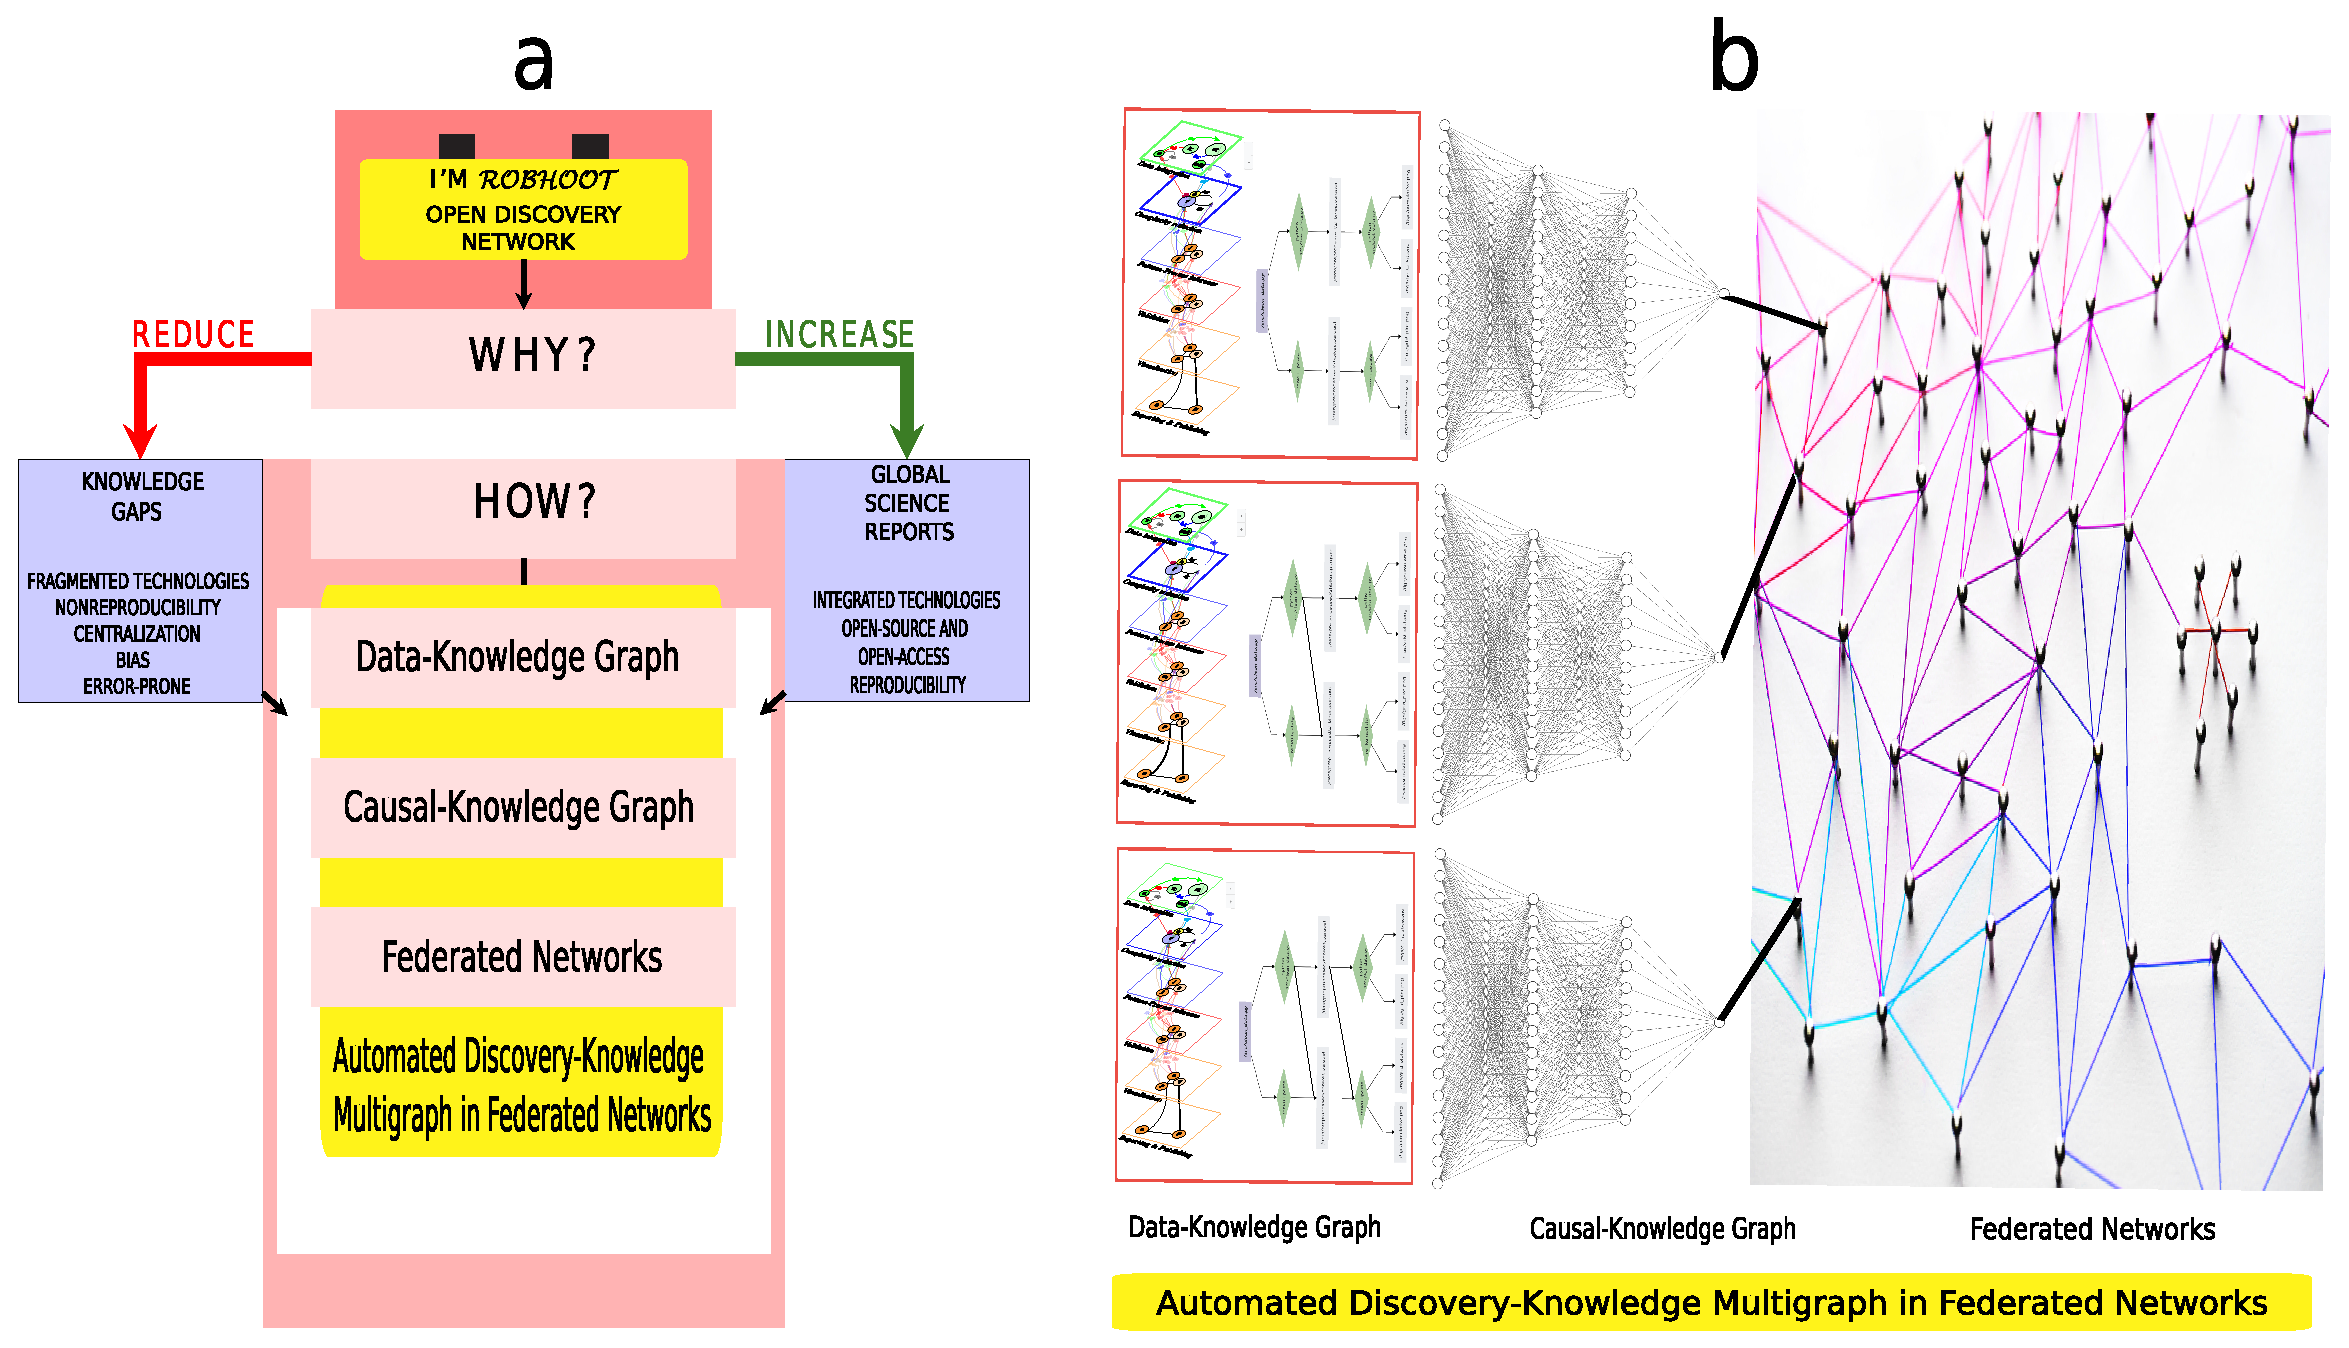
\includegraphics[width=1\textwidth]{Figures/AutomatedDiscovery.pdf}
    \caption*{\small {\bf Figure 1: Discovery-knowledge multigraph
        technology}. $\mathcal{ROBHOOT}$ is an automated federated
      network integrating data- and causal-knowledge graphs, the
      discovery-knowledge multigraph, for a sustainable
      knowledge-inspired society. {\bf a)} $\mathcal{ROBHOOT}$ targets
      global knowledge gaps (red path) and open-access fully
      reproducible discovery reports (green path). It integrates four
      science-enabled technologies: {\bf a,b) Data-Knowledge Graphs}
      for discovering global data-architecture in emergency and
      sustainability landscapes. {\bf a,b) Causal-Knowledge Graphs}
      for automated and explainable biology-inspired neural networks
      discovery. {\bf a,b) Federated Networks} for cooperative
      discovery and forecasting. {\bf Automated Discovery-Knowledge
        Multigraph in Federated Networks} integrate data- and
      causal-knowledge graphs into intelligent federated networks
      technologies for robust cooperative forecasting to rapidly
      respond to global emergency and sustainability challenges.}}
\end{figure}


%--------------------Currently out of the draft
\begin{comment}
 The Robhoot project is trying to introduce new concepts to allow
  scientist and the public to interact in a decentralized open-access
  knowledge network to gain informed decisions when solving complex
  social, environmental and technological problems. Current
  technologies for scientific inquiry are highly fragmented and thus
  only increase robustness, reproducibility and the interactions with
  the public marginally (refs). The goal of Robhoot is to propose a
  new hybrid-technology concept combining deep learning, automation
  and distributed ledger technology with the advances of neural
  biological networks to lay the foundation for a novel open-science
  ecosystem aiming to couple predictive and knowledge power in
  contemporary societies. Robhoot is not set out to deliver a finished
  deep knowledge ledger network in the science ecosystem but provide a
  science-enabled technology in establishing a prototype
  proof-of-principle for an open public-science ecosystem.
 
\begin{table}
 %\rowcolor{pink}
\begin{tabular}{ p{6cm} | p{3cm} | p{3cm}}
  \hline \hline
  \textbf{Features} & \textbf{Science Ecosystem} &\textbf{{\bf $\mathcal{ROBHOOT}$}}\\  \hline
  Decentralization & No & Yes \\ \hline
  Full automation & No & Yes \\ \hline
  Open-access & Mostly No & Yes \\ \hline
  Immutability & No & Yes \\ \hline
  Robustness & Mostly No & Yes \\ \hline
  Reproducibility & Mostly No & Yes \\ \hline        
  Owner-Controlled assets & No & Yes \\ \hline       
  \bottomrule
\end{tabular}
\caption{{\bf $\mathcal{ROBHOOT}$} is designed to resolve desirable
  properties of science: Open-access, immutability, robustness,
  reproducibility, and owner-controlled assets. These features will be
  added during the different stages of development of the project
  (section ``Design Goals'').}
\end{table}
\end{comment}
%-----------------------------------------------------------------

   
\begin{table*}[ht]
 %\rowcolor{pink}
\begin{tabular}{ p{6cm} | p{11cm}}
  \hline \hline
  \textbf{Word} &\textbf{Meaning}\\  \hline
  Question-knowledge graph & Technology-driven information extraction from corpus or similar to detect question gaps in multidisciplinary research\\ \hline
  Data-knowledge graph & Technology-driven information extraction from diverse data-sources to infer global data-architecture \\ \hline
  Causal-knowledge graph & Technology-driven information extraction to provide interpretable scenarios on global and complex sustainability challenges\\ \hline
  % Evidence-based knowledge gap & Solid scientific knowledge facing
  % constraints to be transfered to benefit society\\ \hline
  % Research-based knowledge gap & Differential access to the research
  % knowledge limiting information transfer to the society \\ \hline
  Discovery-knowledge multigraph & Novel interactions emerging from the integration of data- and causal-knowledge graphs to provide multidisciplinary responses to global sustainability challenges\\ \hline
  %Reproducible knowledge graph & High-resolution tracking of the research cycle to make it fully open and transparent\\ \hline
  Automation & Algorithms targeting minimal human-driven interference\\ \hline
  Knowledge-inspired society & Open-access discovery to take informed decisions in global sustainability challenges \\ \hline
  Neutral-knowledge generation & Open reproducible reports making transparent the many sources of bias in the discovery process\\ \hline
  \bottomrule
\end{tabular}
\caption{{\bf Glossary of terms.}}
\end{table*}

\subsection{Science-to-technology breakthrough that addresses this vision}

\begin{itemize}
\item \textcolor{red}{Discuss the relevant state-of-the-art and the
    extent of the advance the project would provide beyond this
    state-of-the-art}
\item \textcolor{pink}{The state-of-the-art of automated and
    interpretable discovery is currently a fragmented and non-compact
    technology. The result is a non-robust and slow response to the
    rapidly growing global emergency and sustainability
    challenges. $\mathcal{ROBHOOT}$ aims to go beyond the
    state-of-the-art in automated and interpretable discovery: First,
    it will fussion automated data- and explainable-knowledge graphs
    into a more compact and robust discovery-knowledge multigraph
    technology. Second, it will fussion discovery-knowledge multigraph
    technology with cooperative federated networks to make a more
    flexible technology to rapidly respond to the growing global
    emergency and sustainability challenges.}
\item \textcolor{red}{Describe the science-to-technology breakthrough,
    targeted by the project that would represent the first proof of
    concept of the envisioned technology}
\item \textcolor{pink}{Patterns from knowledge-graphs are emerging at
    a fast pace, but remains isolated from the full scientific process
    and have been developed in competitive
    environments. $\mathcal{ROBHOOT}$ will go beyond the
    state-of-the-art of knowledge-graphs by developing data- and
    causal-knowledge graphs, the discovery-knowledge multigraphs, in
    cooperative intelligent federated networks to advance
    knowledge-inspired societies towards reaching sustainability
    goals.}
\end{itemize}

Interconnected global societies constantly face new challenges that
need to be rapidly addressed in emerging sustainability
situations. Yet, technologies integrating data-driven causal inference
into intelligent networks providing rapid and global access to robust
information when solving complex governance, social, environmental and
technological problems are particularly lacking. Depite rapid advances
of research platforms for data analytics in the last decade
\citep{Melniketal:2010,Steinruecken,Modulos,Guimera2020,GoogleAI,IrisAI,easeml,datarobot,aito},
the integration of science-to-technology intelligent automation
networks currently lack knowledge-inspired technologies impacting
knowledge-inspired societies to solve global sustainability challenges
(Figure 1 and Tables 1 to 3). In this regard, rapid access to global
API-structured data to perform data-availability analysis, sampling
efforts, heterogeneity and other features to be rapidly integrated to
analyze global data architecture still present challenges (refs). This
is particularly relevant in global emergency or sustainability
landscapes, where data properties like availability, accuracy and
transparency drive questions and scenarios which are constantly
emerging to predict new situations more accurately.

\textcolor{blue}{{\bf $\mathcal{ROBHOOT}$ v.1.0} will deploy a data
discovery technology to generate question- and data-knowledge graphs
for a rapid global understanding of the
data-architecture. Data-architecture alone is not sufficent to make
predictive and plausible scenarios in complex sustainability
situations. Therefore, data analytics complementing data-architecture
discovery and mechanistic inference is desirable to outline plausible
scenarios in rapidly global emerging situations. In this regard, there
are also many gaps in connecting global data-architecture into rapid
automated causal-knowledge graphs to facilitate discovery that can be
transferred to governance decisions. {\bf $\mathcal{ROBHOOT}$ v.2.0} will
integrate automated and explainable biology-inspired neural-networks
to decipher causal-knowledge graphs from open-ended space modeling
scenarios. (Why biologically-inspired neural networks are needed to
build causal-knowledge graphs?) Still, rapidly drawing scenarios from
a few labs limit the phase space from where the discovery process is
generated.(Why data- and causal-knowledge graphs would be explored in
intelligent, federated networks?) The scalability of the discovery
process strongly depends on cooperation and learning protocols in
decentralized networks. Thus, {\bf $\mathcal{ROBHOOT}$ v.3.0} will
explore decentralization and security protocols for discovery in
federated networks (section 3.3), and {\bf $\mathcal{ROBHOOT}$ v.4.0}
will integrate $\mathcal{ROBHOOT}$ v.1.0 to v.3.0 for automated
discovery in global federated cooperation networks.}

\subsection{Interdisciplinarity and non-incrementality of the research
  proposed}

\begin{itemize}
\item \textcolor{red}{Describe the research disciplines necessary for
    achieving the targeted breakthrough of the project and the added
    value from the interdisciplinarity.}
\item \textcolor{red}{Explain why the proposed research is
    non-incremental.}
  \end{itemize}

  {\bf $\mathcal{ROBHOOT}$} is a science-enable multi-feature
  hybrid-technology for automating interpretable data-driven discovery
  in intelligent and cooperative federated networks (Figures 1 and 2
  and Tables 1 and 2). It will contain four modules each characterized
  by a mixture of research disciplines necessary for achieving
  interdisciplinary breakthrough. {\bf $\mathcal{ROBHOOT}$ v.1.0} will
  be compossed by computer scientists and developers targeting API
  discovery protocols and ETLs algorithms. This module will be
  complemented with scientists from the physics of complex networks to
  develop methods for question- and data-knowledge graphs to decipher
  the existing gaps in data discovery and data-architecture
  technologies (section 3.1). {\bf $\mathcal{ROBHOOT}$ v.2.0} team
  will be compossed by data-scientists trained in deep learning
  networks and automation algorithms, theoreticians and biologists
  with expertise in modeling mechanistic and Bayesian networks and
  biology-inspired neural networks. The combination of
  data-scientists, theoreticians and biologists will generate a
  diverse team targeting synthesis between automated and explainable
  biology-inspired neural-networks to decipher causal-knowledge graphs
  from high-dimensional data (section 3.2). {\bf $\mathcal{ROBHOOT}$
    v.3.0} team will be characterized by combining computer scientists
  and developers targeting decentralized protocols (federated
  networks, gnunet), with social scientist, and scientists specialized
  in ecology and evolutionary biology. Team for $\mathcal{ROBHOOT}$
  v.3.0 will explore cooperation protocols for discovery in federated
  networks (section 3.3). Furthermore, the complementarity of the
  teams in the modules one to three will strengthen collaboration
  between the modules for making $\mathcal{ROBHOOT}$ a science-enable
  functional technology in a rapidly evolving digital ecosystem
  \citep{Soto-Valero2019}. {\bf $\mathcal{ROBHOOT}$ v.4.0} team will
  combine computer- and data-scientists working in modules one and
  two, respectively, with developers, biologists, evolutionary
  biologists and social scientists working in modules 2 and 3. Such a
  diverse team will integrate automated and explainable data- and
  causal-knowledge graphs into federated cooperation networks to
  generate automated reporting for global emergency and sustainability
  problems.

  $\mathcal{ROBHOOT}$ aims to bring global transparency in knowledge
  generation by minimizing human intervention to facilitate
  sustainability goals of humanity. This requires a non-incremental
  and multi-feature, science-enabled technology targeting a reduction
  in global knowledge gaps while transparently accounting for
  centralization \citep{Inhaber1977,Gunther2018}⁠⁠, bias⁠⁠
  \citep{Ioannidis2005}, error-prone \citep{Fang2011}, and
  non-reproducibility \citep{Hardwicke2018} (Figure 1 and Table
  1).


  The evolving digital ecosystem is increasing continuously its
  computing capacity (ref Golem+others), new methods accounting for
  automated and explainable AI are rapidly advancing, and their
  interconection to open-source technologies is rapidly occurring in
  the digital ecosystem. Targeting automated data- and
  causal-knowledge discovery in federated cooperative network and
  transfer


  requires the filling
  of many existing technological gaps, from identification and
  retrieval of heterogeneous data sources, to the integration of
  explainable modeling and causal-inference.

  Technologies with the capacity to compactly account for neutral,
  borderless, immutable, and open-access information in hybrid,
  trusted-untrusted peer-to-peer interactions, accounting for the
  multilayer nature of science and engineering are currently not in
  place. We have already advanced in the integration of the different
  modules, from the automated identification, retrieval and data
  integration to inference and process-based discovery. We have
  implemented a prototype for the ongoing covid-19 pandemic (section
  3.3). Each module includes state-of-the-art developments in computer
  science, complex systems, and theoretical evolutionary ecology. The
  proof- of-concept is not fully automated yet and still requires
  human intervention in module integration and the development of a
  testnet stage. Nonetheless, we are currently exploring innovative
  solutions especially in the modules of automated data discovery,
  causal-knowledge graphs, reporting, and visualization.  Producing
  such a technology will require integrating expertise from disparate
  disciplines like multilayer networks, deep learning, automation
  algorithmics, and distributed technologies. The integration of these
  disciplines will require to go beyond domain boundaries.


%Renku, Fabric and gitchain.

\subsection{High risk, plausibility and flexibility of the research approach}


\begin{itemize}
\item \textcolor{red}{Explain how the research approach relates to the
    project objectives and how it is suitable to deal with the
    considerable science-and-technology uncertainties and appropriate
    for choosing alternative directions and options. (The risks and
    mitigation plan should be spelled out under the Implementation
    section).}
\end{itemize}

\section{Impact}

\subsection{Expected impacts}


\begin{comment}
\begin{itemize}
\item \textcolor{red}{Each of the expected impacts listed in the work
    programme:}
\item \textcolor{red}{Scientific and technological contributions to
    the foundation of a new future technology.}
\item \textcolor{pink}{Data-, question-, and causal-knowledge graphs
    will contribute to rapid discovery transfer to the public and
    governance systems.


    facilitate informed decisions in complex problems
    involving human health ecosystems and sustainability
    challenges.


    Question-, data- and causal-knowledge graphs are incipient
    technologies requiring further integration, highly flexible fault-tolerant
    algorithms to access heterogeneous APIs. In addition, inferring
    explainable processes to complex problems would need
    causal-knowledge graphs to obtain the sequence of events that best
    fit to the demography parameters in the Covid-19 at city and
    global scales (i.e., susceptibles, incubation period, infected,
    recovered, and deaths). Generalizing neural (spiking) nets to
    integrate to causal-knowledge graphs extending neural ordinary
    differential/difference methods to rapidly optimize models of
    thousands of parameters.}
\item \textcolor{red}{Potential for future social or economic impact
    or market creation.}
\item \textcolor{pink}{Decision making and governance require the
    built of rapid data-, question-, causal-, and
    reproducible-knowledge graphs to analyze the risks in emergency
    situations to benefit society collectively at local and global
    scales.  For example, the ongoing pandemic is showing us the
    need to account for almost-real-time automated analysis of the
    situation where most of the epidemiological variables are
    unknown. The Asset will assist decision-makers in this regard by
    providing rapid and reproducible reporting accounting for the
    state-of-the-art data and modeling technologies.


    of the risklocal and national health system an automated
    discovery platform using locally collected and standarized data to
    show the importance of rapid and reproducible discovery for
    predicting complex problems at the interface of social and
    governance systems. Specifically, to reach the market, the
    following milestones have been identified: At the end of the first
    year a full operation Asset will be available and tested in a
    human health case study: the propagation of the covid pandemic at
    local and global scales (2y Postdoctoral resercher). During the
    second year, the Asset will be finished with a user-friendly
    interface environment aiming to be useful for the non-expert (6m
    Computer scientist or developer).  }
\item \textcolor{red}{Building leading research and innovation
    capacity across Europe by involvement of key actors that can make
    a difference in the future, for example excellent young
    researchers, ambitious high-tech SMEs or first-time participants 2
    to FET under Horizon 2020}
\item \textcolor{red}{any substantial impacts not mentioned in the
    work programme, that would enhance innovation capacity; create new
    market opportunities, strengthen competitiveness and growth of
    companies, address issues related to climate change or the
    environment, or bring other important benefits for society.}
\end{itemize}

Automated discovery integrating fully reproducible scientific
reporting in federated networks is near to be possible due to the
emergence of open-source technologies in the rapidly evolving digital
ecosystem. Yet, many technologies are highly fragmented and technical
challenges still remain for rapid automated reporting generation to
help taking informed decisions in global emergency situations and
sustainability challenges. 



  
The following are the general and the specific impacts according to
our objectives, working packages and deliverables:

\begin{itemize}
\item Automated knowledge-based network technology\\
  
  The integration between open-source data integration and inference
  schemes, the interlayer automation (O1: Multilayer), will allow for
  the systematic exploration of robust knowledge-based patterns when
  exploring the population of KGs. This is in sharp contrast to
  existing AI technologies mostly oriented to prediction without
  knowledge-based understanding (refs). Despite open-source ETLs are
  rapidly evolving towards accounting for many aspects of data
  integration (formats, historical-real time, storage, dimensions,
  size, bias and spatiotemporal resolution), there is a missing
  component in quantifying the robustness of knowledge that integrated
  data can provide. Automated populations of KGs connecting
  cutting-edge open-source ETLs to inference classification schemes
  can provide the quantification of robustness in knowledge-based
  patters for future predictive technologies.

\item Open immutable knowledge in untrusted digital peer-to-peer ecosystems\\
  
  The open access of immutable accumulation of knowledge in untrusted
  digital peer-to-peer ecosystems: Social, environmental and economic
  impact to facilitate global access to transparent knowledge.  ETLs
  are rapidly evolving towards accounting for many key aspects of data
  integration: Data manipulation across formats (CloverDX), merging of
  historical and real-time streaming data pipelines (i.e., Kafka) and
  data structures facilitating the storage and access of large amounts
  of data (i.e., clickhouse.) Our research methodology will be focused
  on developing an automated workflow using the geographically
  distributed cloud on computing and storage to test the robustness of
  data integration metrics across gradients of simulated data
  containing dimensions, biases, sizes, formats, temporal and spatial
  resolution (should we be more domain specific here? Or should we
  stay general and thinking broadly about simulated data with along
  complexity gradients and explore data integration metrics? How is
  the SDSC dealing with data integration for Renku?  We anticipate
  implementation of an automated end-to-end research cycle within an
  open ledger to facilitate real-time open-access neutral
  data-rule-knowledge to gain informed decisions to help solve complex
  social, environmental and technological problems. This facilitation
  might occur for local, regional and global problems in many
  fronts. Specifically, open deep ledger knowledge networks might have
  an impact in the following five areas
  
\item The identification of gaps in research paths not explored
  consequence of lack of synthesis in interdisciplinary research: The
  creation of new markets opportunities obtained from exploring these
  gaps and the development of comparative method in the science of
  science and citizen data science.

\item The merging of prediction and explanatory power in open science
  to gain synergy between AI open predictive tools and ruled-based
  pattern inference creating a more balanced pattern and process
  inference interaction. Recent examples of AI algorithms playing
  chess and go using brute force deep learning models or rule-based
  algorithms have discovered the power...: The integration between
  prediction and understanding power to facilitate explanatory
  synthesis.

\item The automation of reproducible open knowledge will facilitate
  the reusability, repeatability, and replicability of research
  outputs. The open access knowledge for governance transparency.
  \end{itemize}

\end{comment}
  
\subsection{Measures to maximise impact}

\begin{comment}
  \begin{itemize}
  \item Dissemination and exploitation of results

    1. G4 will launch a testnet to help disseminate the main results
    of the deep ledger knowledge network. The launch will have invited
    NGO’s and GO across disciplines and social, economical and
    technological sectors.

    2. The Robhoot Open network will be launched as a Biodiversity
    research network to integrate the existing public databases and
    crowdsource data collections into the automated KGs and ledger
    network to facilitate NGOs, GO and other organizations
    transparency and governance in Biodiversity management.

    3. The project aims to publish its main findings in top open
    scientific journals to communicate the global impact of a deep
    ledger knowledge network for transparency and governance across
    social and economical sectors.

\item Communication activities

  1. The contribution in communication of the Swiss Data Science Center, Switzerland

  2. Contribution of the Wyss center

  3. Contribution of Ifisc, Spain
\end{itemize}
\end{comment}

\section{Implementation}

\begin{itemize}
\item \textcolor{red}{Describe here the objectives, list of work
    packages, list of deliverables (Ghentt chart)}
\end{itemize}
    
Automating the discovery process to tackle rapid global solutions to
humanity challenges is highly informative by itself, but a diverse
group of scientists across Europe have decided that merely taking
discovery alone is not enough. Science is a highly dynamic and global
process and there are many paths from where it can be achieved. To
understand how discovery broadly, these scientists want to share the
advantages of cooperative discovery in the global digital
ecosystem. To this end, they formed the $\mathcal{ROBHOOT}$ consortium
with the goal of developing a federated network integrating several
technologies into a unified framework. $\mathcal{ROBHOOT}$ will
develop quantitative novel methods such as question-, data-, and
causal-knowledge graphs to understand how cooperative discovery
networks might help towards knowledge-inspired societies to anticipate
global sustainability challenges. This strategy is expected to improve
early access to discovery to rapidly act in emergency global
situations, and indentify new emerging targets where automation and
global reports can play a key role in knowledge-inspired
societies. $\mathcal{ROBHOOT}$'s goals will be developed in four
different stages with sixteen work packages and four main
deliverables.

\subsection{{\bf $\mathcal{ROBHOOT}$ v.1.0}: \\ Data Knowledge Graphs}

\begin{itemize}
      \item \textcolor{red}{Rapid API access to build
          robust and scalable automated interpretable data-driven
          discovery as an existing need. This is particularly relevant
          in global emergency or sustainability landscapes, where new
          questions and scenarios are constantly emerging to predict
          new situations more accurately.}
      \item \textcolor{pink}{Data- and Question-Knowledge graphs as
          solutions for rapid data-driven discovery (defined in Table
          1). Which are their features? Which is the state-of-the-art?
          DKGs will explore similarity patterns of database to
          discover existing gaps in data availability and
          patterns. DKGs will complement QKGs to explore poorly
          explored questions to new pattern discovery.  }
      \item \textcolor{red}{Global and rapid API access to build
          robust and scalable question- and data-knowledge graphs as a
          case study for automated interpretable data-driven
          discovery.}
      \item \textcolor{pink}{Similar to the idea of having a case
          study causal-knowledge graph in the $\mathcal{ROBHOOT}$
          v.2.0, we can represent a data-knowledge graph following the
          Robhack examples.}
      \end{itemize}
      
      Global and rapid access to data to build robust and scalable
      question- and data-knowledge graphs is key for automating
      interpretable data-driven discovery. This is particularly needed
      in emergency or sustainability challenging situations at the
      global scale, where new questions and scenarios are constantly
      emerging. Data access with different privacy requirements,
      formats, heterogeneity, dimensions, bias and spatiotemporal
      resolution is the norm and many projects are rapidly emerging to
      facilitate rapid data access
      \citep{Openstreetmap,Bluecloud,HOT,Elixir}. Yet, available
      automated science-enabled technologies to build data- and
      questions-knowledge graphs at the global scale to rapidly inform
      causal-knowledge graphs about the type of interpretable
      information that can be extracted, while key to make predictive
      scenarios, still remain at a very early stage of development
      despite standard protocols to automate data API access,
      knowledge extraction, and ETFs algorithms are rapidly advancing
      \citep{Fan2012,APISGURU,OpenKnowledgeFoundation}. The
      technologies around automated API data-discovery and
      interpretable question- and data-knowledge graphs remain
      difficult to compactly link to the automated causal-knowledge
      graphs for scientific discovery. $\mathcal{ROBHOOT}$ v.1.0} will
    deploy the following four work packages each with its own
    milestone and a final deliverable: data discovery technology {\bf
      WP1: API discovery (APIDIS)} aiming to build question- {\bf WP2:
      Question-Knowledge graphs (QKGs)} and data-knowledge graphs {\bf
      WP3: Data-Knowledge graphs (DKGs)} and a case study showing how
    merging question- and data-knowledge graphs help to gain
    information about global data-architecture {\bf WP4: Global
      COVID-19 data-architecture (CODA)}.
   
 \begin{figure}[h!]
  %\centering
   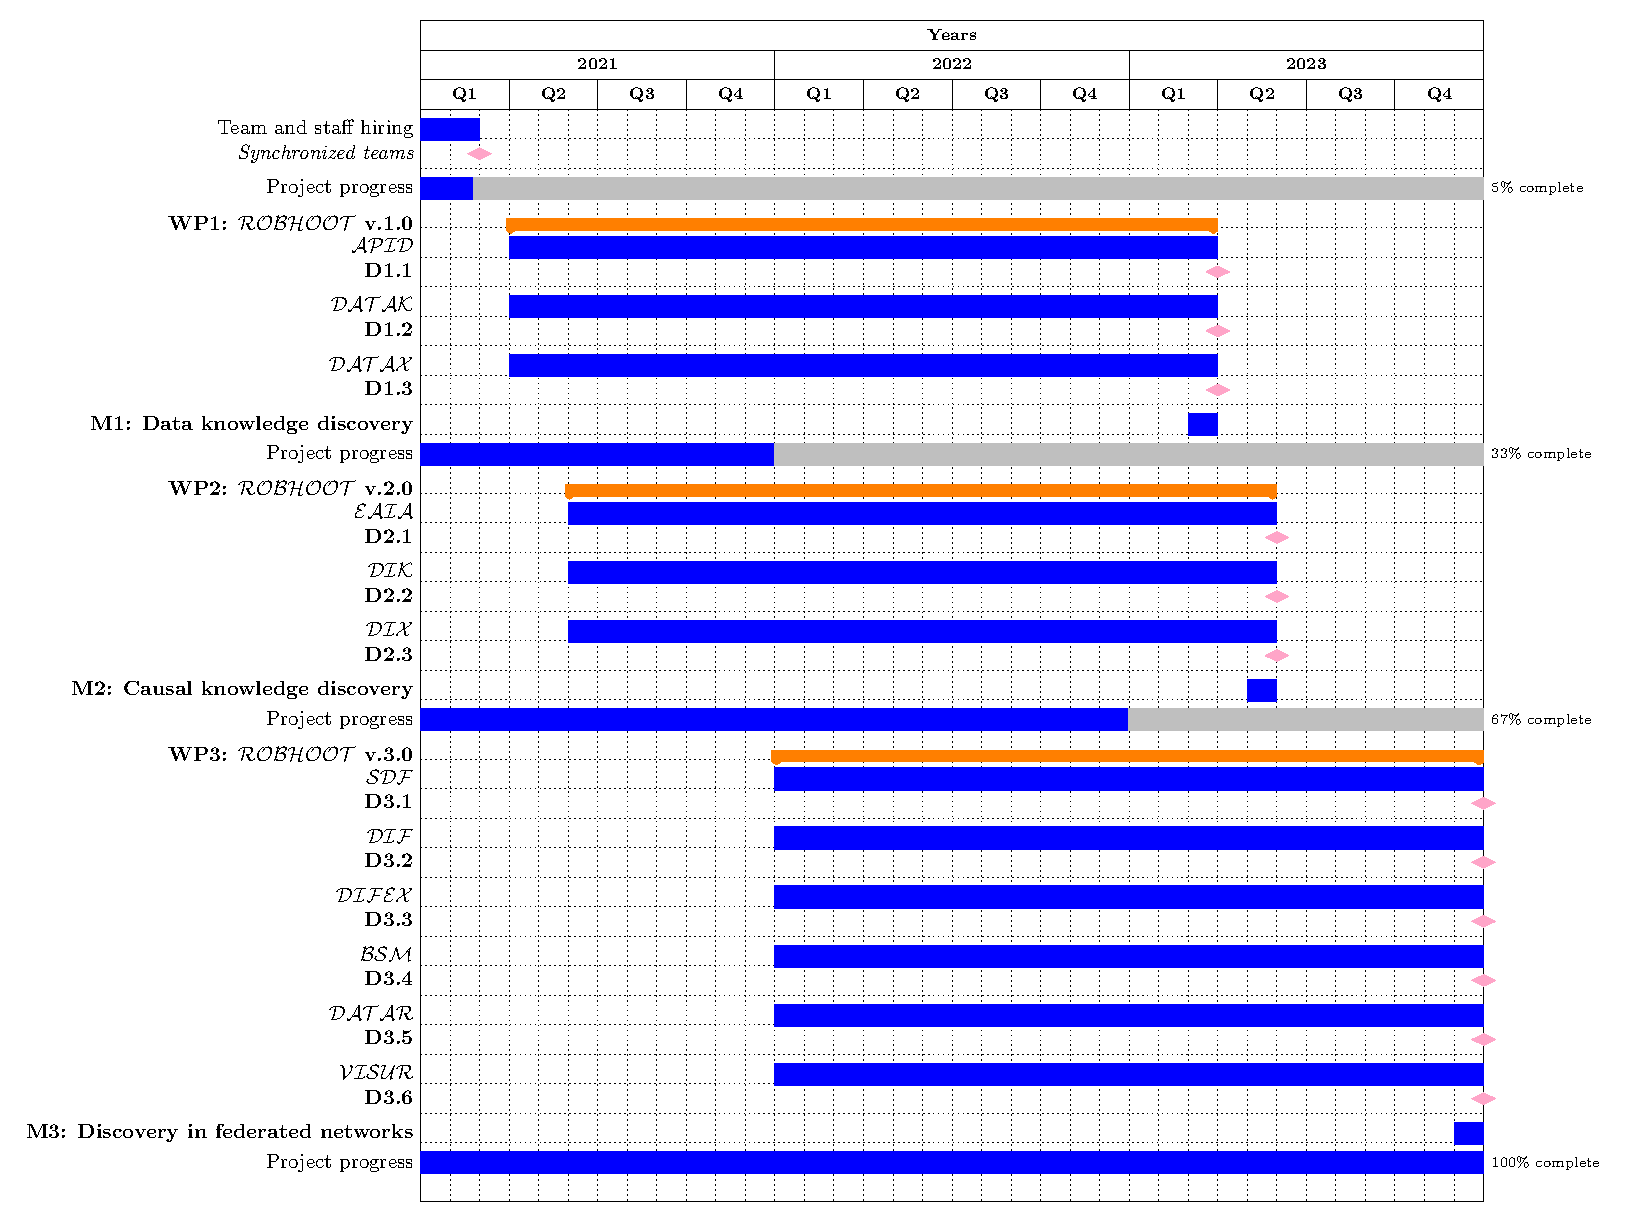
\includegraphics[width=1\textwidth]{Figures/GanttChart.pdf} {\small
     {\bf Figure 2: Roadmap}: {\bf $\mathcal{ROBHOOT}$ v.1.0} work
     packages {\bf WP1} to {\bf WP4} will deploy question-, and
     data-knowledge graphs to decipher global data-architecture
     (Deliverable {\bf D1}). {\bf $\mathcal{ROBHOOT}$ v.2.0} work
     packages {\bf WP5} to {\bf WP8} will develop causal-knowledge
     graphs to merge automation and interpretable data ({Deliverable
       \bf D2}). {\bf $\mathcal{ROBHOOT}$ v.3.0} work packages {\bf
       WP9} to {\bf WP12} will develop cooperative forecasting
     protocols in federated networks aiming to generate global access
     reports in face of rapidly emerging global emergency and
     sustainability challenges (Deliverable {\bf D3}), and {\bf
       $\mathcal{ROBHOOT}$ v.4.0} work packages {\bf WP13} to {\bf
       WP16} will deploy automated discovery-knowledge graphs in
     federated networks.}
\end{figure}


\subsection{{\bf $\mathcal{ROBHOOT}$ v.2.0}: \\ Causal Knowledge Graphs}

  \begin{itemize}
  \item \textcolor{red}{Contrasting explainable biologically inspired
      Causal Knowledge Graphs to quantify the reproducibility,
      reusability, and recovery properties of discovery}
   \item \textcolor{pink}{WP5: Causal Spiking Neural Networks (CSNN)}
   \item \textcolor{red}{Conntrasting predictions from Causal Spiking
       Neural Networks in the framework of Bayesian Space Models to
       explore open-ended language of models combining Bayesian
       networks and optimization methods}
   \item \textcolor{pink}{WP6:Bayesian Space Models (BSM)}
   \item \textcolor{red}{Case study}
   \item \textcolor{pink}{Covid-19 Causal Knowledge Graph}
   %\item \textcolor{red}{}
   %\item \textcolor{pink}{}
   \end{itemize}

   AI is rapidly advancing in automated discovery (i.e., AutoML
   \citep{Real2020}) making more transparent the processes underlying
   the discovery (i.e., Explainable or interpretable AI
   \citep{Gil2019,Futia2020}). Yet, both automated and explainable
   discovery methods are still at an incipient stage of integration,
   particularly in open-ended Bayesian machines
   \citep{Guimera2020}. This is particularly relevant in the context
   of biology, brain research, and evolutionary biology techniques
   where making automatic interpretation of complex systems can
   provide scenarios to help disentangling complex sustainability
   problems for humanity. $\mathcal{ROBHOOT}$ v.2.0 will develop novel
   causal knowledge graphs integrating automated and explainable
   discovery accounting for biologically inspired neural networks and
   evolutionary biology techniques
   \citep{Maass2014,Maass2015}. Automatic interpretation of the causal
   processes underlying empirical patterns will be explored in a
   series of neuromorphic computing scenarios using neural networks of
   evolving spiking neurons ({\bf WP5: Causal Spiking Networks (CSN)}
   (Figure 2).

   Causal Spiking Neurons will explore open-ended language of models
   with varying biologically relevant functions like code insertions,
   deletions, inversions and other molecular and genotype-phenotype
   processes to search for automated biologically inspired solutions
   to complex empirical patterns {\bf WP6: Automated Causal Knowledge
     Graphs (ACKG)}. Causal knowledge graphs will help to enhance the
   connection between automated and explainable AI throughout
   prediction and knowledge power (Figure 3). Automated and
   interpretable data inference still present many challenges in the
   context of multidimensional landscapes
   \citep{OHare2015,Cranmer2019}. This is particularly relevant in
   Earth and Ecosystem science \citep{Reichstein}, where merging
   automation to interpretable data will increase human ability to
   make stronger inferences about future sustainability challenges and
   solutions. In order to make inference from complex data more robust
   we will contrast predictions from Causal Spiking Networks in the
   framework of Bayesian Space Models to explore open-ended language
   of models combining Bayesian networks and optimization methods
   ({\bf WP7: Bayesian Space Models (BSM)}. The Bayesian space models
   module will ensure the search, the evaluation of models,
   trading-off complexity, fitting to the data and quantify resource
   usage \citep{Guimera2020,Steinruecken}. $\mathcal{ROBHOOT}$ v.2.0
   will deploy the COVID-19 pandemic as a case study to automatically
   infer locally interpretable causal-knowledge graphs a global scale
   ({\bf WP8: COVID-19 Causal-Knowledge Graphs (COCAUS)}).

 \begin{figure}[h!]
   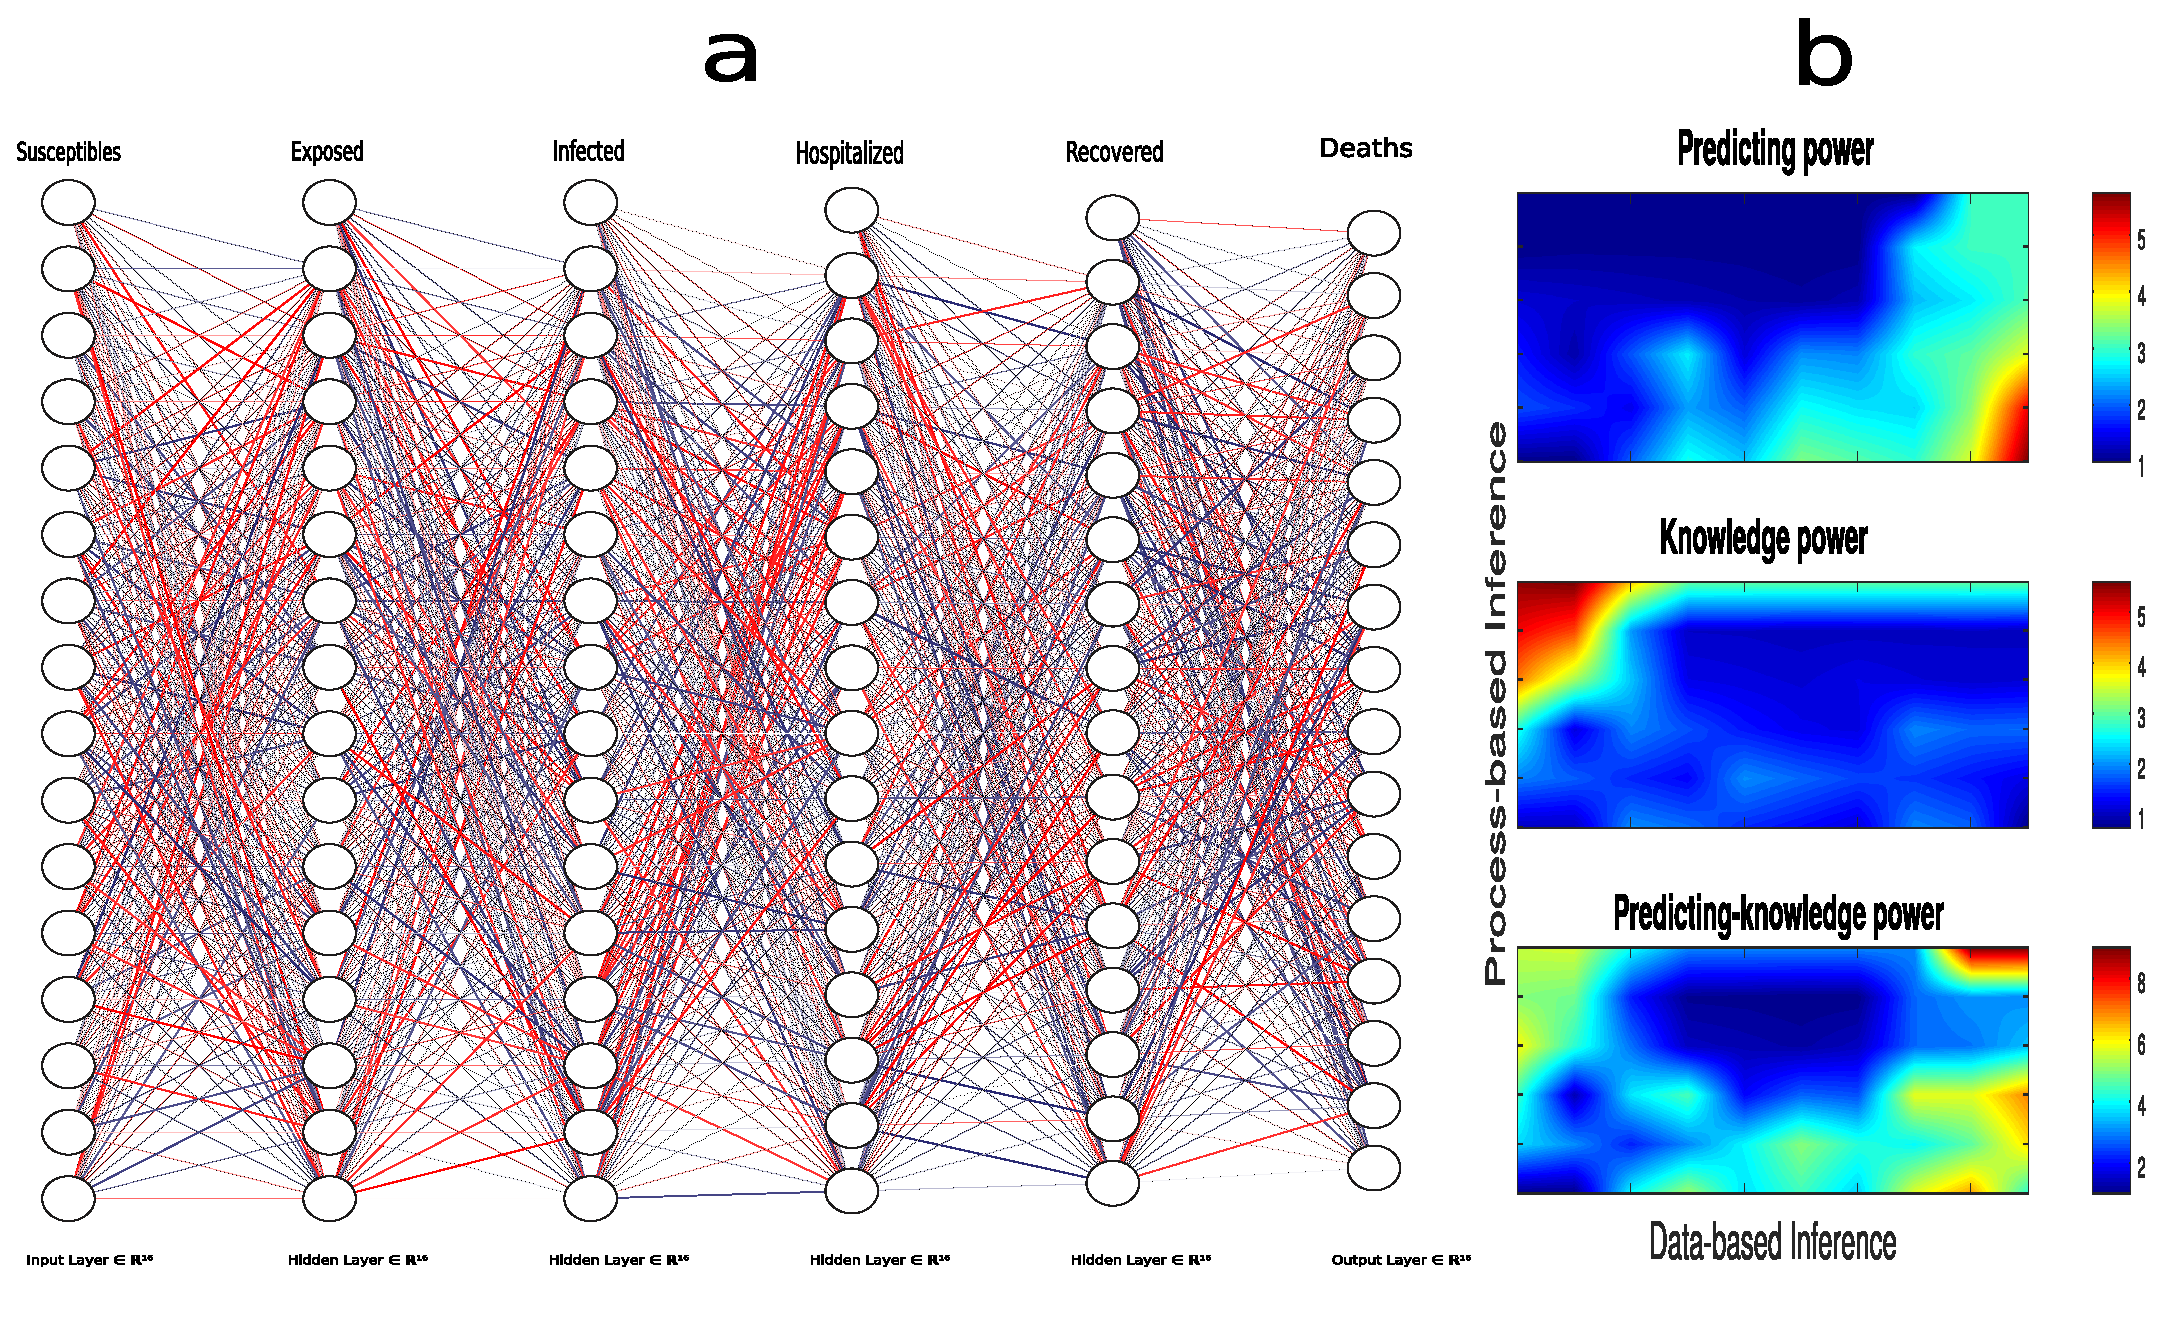
\includegraphics[width=1\textwidth]{Figures/Figure3integrated.pdf}
   {\small {\bf Figure 3: Prediction-explainable power map in
       Automated Causal Knowledge Graphs}. {\bf A}) Automated Causal
     Knowledge Graphs contain features to ... {\bf B)} x-axis
     represents data-based inference (i.e., gradient of AI methods
     from low (left) to high (right) predictive power). y-axis
     represents process-based inference (i.e., gradient of
     process-based methods from low (bottom left) to high (top left)
     understanding power). The gradient of predicting power map (top)
     shows a hot spot red area in the bottom right highlighting the
     region where AI methods best predict the empirical data. The
     gradient of understanding power map (middle) shows a red hot spot
     in the top left highlighting the region where the best
     mechanistic understanding occur. The predicting-understanding
     power map (bottom) shows the sum of the two previous maps
     highlighting a red hot spot where the best synthesis research
     joining predicting and understanding power of the empirical data
     might occur. The first research goal of this proposal aims to
     build an automated research platform to maximize the predicting
     and understanding power highlighted in the red hot spot of the
     predicting-understanding power map (bottom).}
\end{figure}
  
  
\subsection{{\bf $\mathcal{ROBHOOT}$ v.3.0}: \\ Federated Networks}

  \begin{itemize}
  \item \textcolor{red}{A science-based automated and explainable
      technology is not enough if we aim to globally contrast robustly
      paths for automatic interpretation of causal processs predicting
      the empirical patterns.}
  \item \textcolor{pink}{A science-based technology to efficiently
      develop cooperative forecasting aiming to find robust
      populations of results in face of rapidly emerging global
      emergency and sustainability challenges.}
  \end{itemize}

  A science-based automated and explainable technology is not enough
  if we aim to globally contrast robustly paths for automatic
  interpretation of causal processes predicting the empirical
  patterns. Efficient information sharing protocols are needed to
  develop scalable cooperative forcasting and strong
  inference. $\mathcal{ROBHOOT}$ v.3.0 will focus on the extension and
  development of protocols in digital networks to embed automated and
  explainable discovery-knowledge graphs into global cooperation
  schemes to increase robustness, reproducibility, decentralization
  and rapid reporting generation \citep{Dilley2016}. Technologies in
  decentralized digital ecosystems is rapidly advancing in a variety
  of sectors. Most progress is coming in the scalability, security and
  decentralization trade-offs
  \citep{Golem2016,Dilley2016,Durov2017,Androulaki2018,OceanProtocolFoundation2018,BigchainDBGmbH2018}. In
  the open science ecosystem, only a few implementations of
  decentralized technologies exist \citep{Gunther2018}.

  $\mathcal{ROBHOOT}$ v.3.0} will deploy the following four work
packages each with its own milestone and a final deliverable: sharing
question-, and data-knowledge graphs, the data-architecture, in
federated networks using reproducible-knowledge graphs {\bf WP9:
  Sharing data-architecture in federated networks (SDFN)}. Sharing
causal-knowledge graphs in federated networks using
reproducible-knowledge graphs {\bf WP10: Sharing causal-knowledge
  graphs in federated networks (SCFN)}. Sharing data-architecture and
causal-knowledge graphs in federated networks using
reproducible-knowledge graphs {\bf WP11: Sharing data-architecture and
  causal-knowledge graphs in federated networks (SDCFN)}. The last
work package of $\mathcal{ROBHOOT}$ v.3.0, {\bf WP12: Sharing
  data-architecture and causal-knowledge graphs in federated networks
  COVID-19 case study (SDCFNCO)}, will deploy sharing
data-architecture and causal-knowledge graphs in federated networks
for the COVID-19 case study. Despite recent decades have seen a
dramatic rise in global pandemics (i.e., the SARS pandemic in 2003, to
Avian Influenza in 2006, H1N1 in 2009, Ebola in 2014, the appearance
of the Zika virus in Latin America in 2015, and the current Covid-19
pandemic), and these developments are inextricably bound up in modern
socio-technical developments and processes of globalization,
science-based technologies facilitating rapid sharing of information
and automation to mitigate risks and enhance response efficiency with
globally informed scenarios are particularly lacking
\citep{Wilson2018}.
 
  \subsection{{\bf $\mathcal{ROBHOOT}$ v.4.0}: \\ Automated
    Discovery-Knowledge Graphs in Federated Networks}

  \begin{itemize}
  \item {\bf WP13: ADADI}{28}{38}\\%Automated data-discovery federated
                                   %network
  \item {\bf WP14: ACADI}{28}{38}\\%Automated causal-discovery
    % federated network
  \item {\bf WP15:
      ADACADI}{28}{38}\\%Automated data-causal-discovery federated network
  \item {\bf WP16:
      ADACADICO}{36}{42}\\%Cooperative forecasting in automated-discovery-knowledge graphs for the COVID-19 case study
  \end{itemize}
  
\begin{comment}
  \begin{itemize}
  \item Deployment of a permissioned-permissionless distributed ledger
    technology to guarantee decentralization, open-access,
    neutral-knowledge-based network generation and prior
    confidenciality/posterior reproducibility of the KGs populations
    (Figures 2c and 2d).
  \item Exploration of a suite of consensus algorithms and smart
    contracts among trusted-untrusted peer-to-peer interactions to
    infer macroscopic metrics of the open research network (Figure
    2d).
  \item Quantification of metrics to study the
    scalability-security-decentralization trade-offs when storing KGs
    in the research network (Figure 2d).
  \item Testnet case study to explore the interaction between
    consensus protocols and the scalability-security-decentralization
    trade-offs when committing the KGs to the distributed ledger.
  \item Mainnet to cryptographically link each population of KGs to
    previous KGs-ledger to create an historical KGs-ledger chain that
    goes back to the genesis ledger of the open research
    network. Launching of the mainnet to connect multiple database
    integration with real-time open-access citizen data science and
    knowledge-inspired societies.
  \end{itemize}

   \begin{itemize}
   \item {\bf Tools and Methods}: Distributed computing algorithms,
     Blockchain and consensus algorithms, BighainDB,
     Gitchain. Telegram open network, Golem.
 \end{itemize}

 \begin{itemize}
 \item {\bf Novel Territory}: Deployment of contrasting functional
   consensus algorithms to explore decentralization and robustness
   properties of the KGs populations along ensembles of the research
   cycle space.
   \end{itemize}
  

\begin{table*}[ht]
 %\rowcolor{pink}
\begin{tabular}{ p{3.5cm} | p{14cm}}
  \hline \hline
  \textbf{Feature} &\textbf{$\mathcal{ROBHOOT}$}\\  \hline
  Long-term vision & Global open-access to a fully reproducible knowledge-generation inspired technology \\ \hline
  Breakthrough scientific and technological target & Collapsing evidence- and research-based knowledge gaps for a sustainable knowledge-inspired society\\ \hline
  Novelty & Science-based technology emerging from targeted algorithmic discovery at the interface of multilayer networks, knowledge graphs, deep-learning, and consensus mechanisms\\ \hline
  Foundational & Neutral-knowledge inspired technology for an emerging open science of science and science-society research disciplines \\ \hline
  High-risk & Adapted to explore new terrirories into the open-science-technology-society interface ecosystem \\ \hline
  Interdisciplinarity & Hybridizing expertise from distributed computing and deep learning to multilayer networks and the ecology and evolution of natural and digital ecosystems (Table 1) \\ \hline
  \bottomrule

\end{tabular}
\caption{{\bf $\mathcal{ROBHOOT}$} features along its developmental stages.}
\end{table*}
\end{comment} 

\begin{comment}
The science ecosystem requires multiple steps of information transfer
among trusted/untrusted peers. In this ecosystem, immutable and secure
peer-to-peer architecture storing end-to-end open-source research is
key to have neutral access to full reports to gain informed decisions
in complex societal, environmental and technological problems. The
overall objectives for the project with the outlines of the specific
goals of each one are the following:

\begin{item}
\item Deploy an automated knowledge-based network technology
  accounting for end-to-end research in a lineage client-tracker to
  produce a population of Knowledge Graphs (KGs) (Figures 1a-b.)
\item Intralayer automation of data integration, inference, and
  validation (Figure 1a.)
\item Intralayer automation of visualization and reporting generation
  (Figure 1a.)
\item Deep intra- and inter-layer automation with a lineage
  client-tracker paths in the multilayer network (Figures 1a-c.)
\item Deploy an end-to-end permissioned-permissionless distributed
  ledger technology to guarantee decentralization, open-access and
  security of the KGs in the science ecosystem (Figures 1c and 1d.)
  \item Distributed ledger implementation accounting for consensus
    algorithms and smart contracts among trusted-untrusted
    peer-to-peer interactions.
  \item Exploring scenarios to minimize
    scalability-security-decentralization trade-offs when storing the
    KGs in the science ecosystem
  \item DeepKlen, a deep knowledge ledger network, to explore the
    interaction between consensus protocols, the
    security-scalability-decentralization trade-offs and the
    robustness of the generated KGs in the automated science
    ecosystem.
  \item Testnet for the interaction between consensus protocols and
    the scalability-security-decentralization trade-offs when
    reporting the KGs to the ledger.
  \item Mainnet to cryptographically link each population of KGs to
    previous KGs-ledger to create an historical KGs-ledger chain that
    goes back to the genesis ledger. The mainnet aims to connect
    real-time open-access citizen data science to knowledge-inspired
    societies.
  \item Robhoot Open Network in Biodiversity Research to connect
    citizen open science to real-time open-access data-rule-knowledge
    to gain informed decisions when solving local and global
    environmental problems.
  \item Citizen open science for biodiversity datasets integration
    (Figure 1a top layer and Figure X)
  \item Testnet for Biodiversity research in a deep knowledge ledger
    network (Figure 2.)
\end{item}

The science ecosystem currently lack technologies fully automating the
research cycle into the open-source digital ecosystem. Despite public
institutions are demanding more reproducibility and openness of the
data and the scientific process, and overall a shifting towards open
and reproducible scientific and engineering landscapes, there are not
currently open and integrated technologies aiming to compactly
facilitate and distribute the scientific and engineering knowledge in
open, reproducible and immutable knowledge networks (Tables 1 and 2).
  
  Automating knowledge-generation requires the integration of many
  distinct features. Usually, knowledge-generation comes from
  interactions within- and between-layers of the scientific process
  (Figure 2a). The feedbacks occurring within and among layers in the
  science and technology ecosystem also provide unexpected behaviors
  that are difficult to anticipate. Therefore many feedbacks and
  interactions within- and between-layers are not easy to reproduce if
  not properly accounted for. We will take advantage of the
  open-source software community to explore knowledge graphs,
  optimization, automation, and decentralization algorithms together
  to study the robustness and reproducibility properties of the
  scientific process (Figures 1 and 2).

  One way of visualizing the dimensionality of $\mathcal{ROBHOOT}$ in
  the digital ecosystem is to connect each layer of the scientific
  process (Figure 2a) to open-source software to gain functionality of
  the open research network (Figure 3). For example, Node 0 (left
  column, Figure 3) can be the Data Integration layer in Figure
  2a. This node is connected to seven nodes representing open-source
  ETLs open-source software (i.e., central column, Figure
  3). Connections between Node 0 and nodes 5, 6, 8, 9, 10, 12 and 13
  can be rapidly evolving (i.e., indicated by the different red tones
  of the connections). Indeed, open-source ETLs are rapidly evolving
  towards accounting for many heterogeneous aspects of data
  integration (i.e., formats, historical-real time, storage,
  dimensions, size, bias and spatiotemporal resolution). ETLs can also
  be connected to a gradient of reporting generation (i.e., right
  column, Figure 3) noting reports containing only a subset of the
  interactions of the digital ecosystem network. The network of the
  fully automated research cycle can be one where Nodes 0, 1, 2, 3,
  and 4 represent the different layers of the research cycle (left
  column, Figure 3 and Figure 2a) connected to the open-source
  software of the digital ecosystem (central column, Figure 3) to
  generate full populations of reports (right column, Figure 3).
\end{comment}
  
  \begin{comment}
    %\centering
  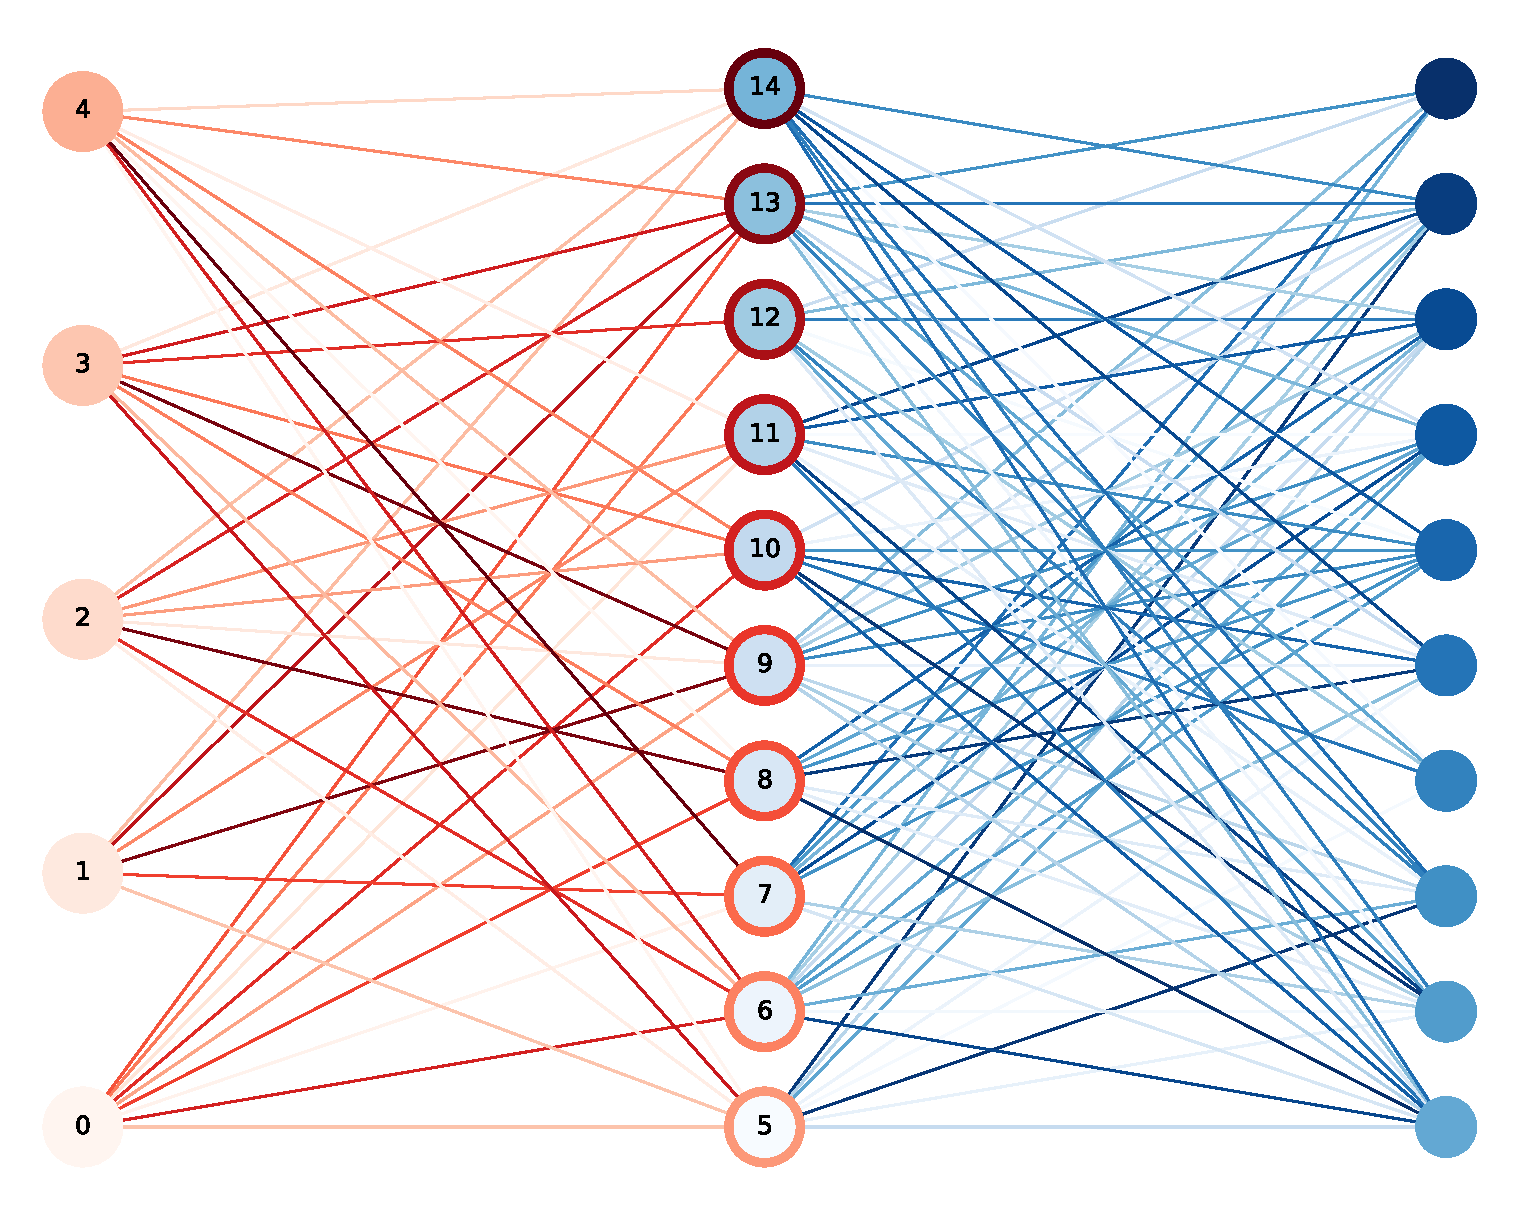
\includegraphics[width=0.45\textwidth]{Figures/FigureRobhoot.pdf}
 
  {\small {\bf Figure 3: Robhoot in Digital Ecosystems}: {\bf Left
      column}: {\bf $\mathcal{ROBHOOT}$ v.1.0} representing the
    research cycle as nodes from number 0 to 4: Data integration (0),
    Complexity Reduction (1), Inference (2), Validation (3), and
    Visualization(4)). {\bf Central column}: Nodes representing the
    research cycle in the left column are connected to open-source
    software in the digital ecosystem. Connections with node number 0
    in the left column can, for example, represent the ETLs
    open-source software interactions required to generate the {\bf
      Universal ETLs} module. The same meaning applies to the
    different nodes of the left column. {\bf Right column}: Each node
    represents a report meaning there is a reporting gradient
    generated by the connections to the open-source software from
    where each report is generated only using a subset of the research
    layers and open-source software.}
\end{comment}

  
\subsection{Research methodology and work plan – Work packages,
  deliverables}

\begin{comment}
The research methodology and work plan contains 16 work packages each
with its respective milestone and 4 deliverables (Gantt and PERTH
charts, Figures 2 and 3 respectively). The following 

and Box 2. Box 1 highlights a preliminary analysis of our source data
in the road to infer the number of layers. Box 2 describes the deep
process- based learning networks scenarios to infer the strength of
the feedbacks between the layers in the data. Sections 4.2 and 4.3
describe the sampling features of our source data and the
collaboration with the SDSC to achieve the planned work packages, the
milestones and the deliverables.  4.2 Data


4.3 Collaboration with the SDSC for the Work Packages, Milestones and
Deliverables
The team will be composed by the SDSC, the MAIN (Carlos Melián) and the CSYS (Victor
Eguíluz) to produce one methods package and two scientific papers during the development of
the proposal. Below we describe the timeline describing the milestones, the deliverables, the
timing to release the packages in public repositories and the scientific papers (Table 1).
Work packages
WP1: Data visualization
Leading groups: MAIN and CSYS; Contributed data: GEN, ECO, BIOD and RIV
WP2: Multilayer inference in the multidimensional data (Box 1 and Section 4.2)
Leading groups: SDSC, MAIN and CSYS; Contribution: GEN, ECO, BIOD and RIV
WP3: Deep process-based learning networks in biodiversity research (Box 2)
Leading groups: SDSC, MAIN, and CSYS.
Milestones
M1.1: Uploading the Projet Lac database, the Progetto Fiumi, the Whitefish community
database, and the Threespine Stickleback database to the SDSC platform.
M1.2: Visualization of the empirical data in multilayer networks using existing software.
M2.1: Public animation exhibition: Visualization showing our source data in a permanent
exhibition hosted by the Natural History Museum in Bern. The animations will be featuring the
Fish communities in the rivers and lakes of Switzerland. The animations will highlight the
interactions from genes to landscapes integrating genetic, phenotypic, ecological and spatial
data. Please check https://www.nmbe.ch/de/unser-angebot/unser-angebot/fuer-forschende/
wirbeltiere section Ichthyologie with Projet Lac being one of the projects contributing the
most to the current FishEc database and https://www.nmbe.ch/de/museum/aktuelles/monster-
im-saft for the status of this permanent exhibition.
M3.1: Multilayer inference from multidimensional data (Box 1).
M3.2: Synthesis of methods for multilayer inference.
M4.1: Implementation of deep process-based learning networks scenarios (Box 2).
M4.2: Contrasting biodiversity patterns with and without feedbacks in multilayer networks.

4.1 General description of the scientific approach
We outline our research plan in Box 1 and Box 2. Box 1 highlights a preliminary analysis of
our source data in the road to infer the number of layers. Box 2 describes the deep process-
based learning networks scenarios to infer the strength of the feedbacks between the layers in
the data. Sections 4.2 and 4.3 describe the sampling features of our source data and the
collaboration with the SDSC to achieve the planned work packages, the milestones and the
deliverables.
4.2 Data
\end{comment}

\begin{comment}
  \textcolor{red}{3. Implementation 3.1 Research methodology and work
    plan – Work packages, deliverables We will use a hybrid modular
    approach (refs for selecting project management) containing four
    objectives, eleven work packages and X deliverables. The following
    is the research methodology and timing of the work packages and
    the connections among the packages within and across goals: O1:
    Multilayer WP1 (ADAI): Automated data acquisition and
    integration. Open-source ETLs are rapidly evolving towards
    accounting for many key aspects of data integration: Data
    manipulation across formats (CloverDX), merging of historical and
    real-time streaming data pipelines (i.e., Kafka) and data
    structures facilitating the storage and access of large amounts of
    data (i.e., clickhouse.) Our research methodology will be focused
    on developing an automated workflow using the geographically
    distributed cloud on computing and storage to test the robustness
    of data integration metrics across gradients of simulated data
    containing dimensions, biases, sizes, formats, temporal and
    spatial resolution (should we be more domain specific here? Or
    should we stay general and thinking broadly about simulated data
    with along complexity gradients and explore data integration
    metrics? How is the SDSC dealing with data integration for Renku?
    MapReduce Golem network Resource distribution in data storage and
    simulating data (Ease.ml constraints and novelty and how Fluence
    network can help to solve it) WP2 (PROPANCE): Process pattern
    automated inference. Automated classification scheme to explore
    many inference methods across the population of KGs.  WP3 (VISUR):
    Intralayer visualization and reporting. We will integrate and
    develop new algorithms to merge distinct database into one large
    db using mySQL, clickhouse or similar db-open-source software.
    WP4 (XX) Multilayer and KG integration: Existing knowledge of
    neural networks (refs by Luis) and deep knowledge-based algorithms
    to obtain the KGs (integrating WP1-3.)  automated ledger knowledge
    network technology to compactly facilitate open-science,
    decentralization, reproducibility and security in the science
    ecosystem O2: Ledger WP5 (): DeepKlen consensus protocol (DCP).
    The ledger represents the DeepKlen universe at a given point in
    time. It contains the KGs list and all the orders in the
    distributed network. We will define and implement a protocol to
    which KG set to apply to the last ledger.  WP6 (): Scalability,
    decentralization and security protocols.  WP7 (): Ledger
    automation O3: DeepKlen WP8 (): Testnet WP9 (): Mainnet O4:
    Robhoot WP10 (): Testnet Showcase of the julia packages to be
    integrated within and between layers and the existing gaps.  WP11
    (): The Robhoot Open Network (RON) for Biodiversity research}
\end{comment}
  
  \subsection{Management structure, milestones and procedures}
  \begin{itemize}
  \item \textcolor{red}{Describe the organisational structure and the
      decision-making (including a list of milestones (table 3.2a))}
\item \textcolor{red}{Explain why the organisational structure and
  decision-making mechanisms are appropriate to the complexity and
  scale of the project.}
\item \textcolor{red}{Describe any critical risks, relating to project
    implementation, that the stated project's objectives may not be
    achieved. Detail any risk mitigation measures. Please provide a
    table with critical risks identified and mitigating actions (table
    3.2b) and relate these to the milestones.}
  \end{itemize}

  \subsection{Consortium as a whole}

  \begin{itemize}
    \item \textcolor{red}{The individual members of the consortium are
        described in a separate section 4}
      \item \textcolor{red}{Describe the consortium. Explain how it will
    support achieving the project objectives.  Does the consortium
    provide all the necessary expertise? Is the interdisciplinarity in
    the breakthrough idea reflected in the expertise of the
    consortium?}
\item \textcolor{red}{In what way does each of the partners contribute
    to the project? Show that each has a valid role and adequate
    resources in the project to fulfil that role. How do the members
    complement one another? Other countries and international
    organisations: If one or more of the participants requesting EU
    funding is based in a country or is an international organisation
    that is not automatically eligible for such funding (entities from
    Member States of the EU, from Associated Countries and from one of
    the countries in the exhaustive list included in General Annex A
    of the work programme are automatically eligible for EU funding),
    explain why the participation of the entity in question is
    considered essential for carrying out the action on the grounds
    that participation by the applicant has clear benefits for the
    consortium.}
  \end{itemize}


  \subsection{Resources to be committed}
 
  \begin{itemize}
  \item \textcolor{red}{Please make sure the information in this
      section matches the costs as stated in the budget table in
      section 3 of the administrative proposal forms, and the number
      of person months, shown in the detailed work package
      descriptions.  Please provide the following:}
 \item \textcolor{red}{a table showing number of person months required
    (table 3.4a)}
  \item \textcolor{red}{a table showing ‘other direct costs’ (table
      3.4b) for participants where those costs exceed 15\% of the
      personnel costs (according to the budget table in section 3 of
      the administrative proposal forms)}
\end{itemize}


\begin{comment}
\section{Their relevance in terms of Future and Emerging Technologies}

Table 2 

\subsection{Scientific concept}
Research cycle automation combining novel decentralization algorithms
with data, inference, and knowledge graphs integration

\subsection{Identified problem}
Global sustainability  is a major goal of humanity. Many studies have
shown global sustainability could be achieved by strengthening
transparency and feedbacks between social, ecological and governance
systems. Sustainability goals, however, strongly depend on global
society access to evidence- and research-based knowledge gaps. Yet,
the science ecosystem lacks open-source technologies narrowing down
the different aspects of knowledge gaps.


\subsection{Potential solutions envisaged}
\begin{itemize}
\item Global access to fully reproducible reports
\item Testnet case study in Sustainability and Biodiversity research to facilitate open an global access  
\end{itemize}

\subsection{Describe the vision of a radically-new science-enabled}


\subsection{Technology that the project would contribute towards}

\textcolor{red}{Implementation 3.1 Research methodology and work plan
  – Work packages, deliverables We will use a hybrid modular approach
  (refs for selecting project management) containing four objectives,
  eleven work packages and X deliverables. The following is the
  research methodology and timing of the work packages and the
  connections among the packages within and across goals: O1:
  Multilayer WP1 (ADAI): Automated data acquisition and
  integration. Open-source ETLs are rapidly evolving towards
  accounting for many key aspects of data integration: Data
  manipulation across formats (CloverDX), merging of historical and
  real-time streaming data pipelines (i.e., Kafka) and data structures
  facilitating the storage and access of large amounts of data (i.e.,
  clickhouse.) Our research methodology will be focused on developing
  an automated workflow using the geographically distributed cloud on
  computing and storage to test the robustness of data integration
  metrics across gradients of simulated data containing dimensions,
  biases, sizes, formats, temporal and spatial resolution (should we
  be more domain specific here? Or should we stay general and thinking
  broadly about simulated data with along complexity gradients and
  explore data integration metrics? How is the SDSC dealing with data
  integration for Renku?  MapReduce Golem network Resource
  distribution in data storage and simulating data (Ease.ml
  constraints and novelty and how Fluence network can help to solve
  it) WP2 (PROPANCE): Process pattern automated inference. Automated
  classification scheme to explore many inference methods across the
  population of KGs.  WP3 (VISUR): Intralayer visualization and
  reporting. We will integrate and develop new algorithms to merge
  distinct database into one large db using mySQL, clickhouse or
  similar db-open-source software.  WP4 (XX) Multilayer and KG
  integration: Existing knowledge of neural networks (refs by Luis)
  and deep knowledge-based algorithms to obtain the KGs (integrating
  WP1-3.)  automated ledger knowledge network technology to compactly
  facilitate open-science, decentralization, reproducibility and
  security in the science ecosystem O2: Ledger WP5 (): DeepKlen
  consensus protocol (DCP). The ledger represents the DeepKlen
  universe at a given point in time. It contains the KGs list and all
  the orders in the distributed network. We will define and implement
  a protocol to which KG set to apply to the last ledger. WP6 ():
  Scalability, decentralization and security protocols.  WP7 ():
  Ledger automation O3: DeepKlen WP8 (): Testnet WP9 (): Mainnet O4:
  Robhoot WP10 (): Testnet Showcase of the julia packages to be
  integrated within and between layers and the existing gaps. WP11 ():
  The Robhoot Open Network (RON) for Biodiversity research}

\subsection{Describe how this vision surpasses paradigms that
  currently exist}


\subsection{Overall and specific objectives for the project}
\textcolor{red}{High risk, plausibility and flexibility of the
  research approach\\ We are in need of accounting for the
  uncertainties, the reproducibility and immutability related to
  automation in science and engineering. This need is not just for a
  specific stage of the research cycle, but for the full research
  cycle, from data acquisition to reporting generation because
  knowledge-inspired societies and governance will demand full
  research cycle transparency in solving complex social, environmental
  and technological problems. This need brings many challenges to our
  research proposal because obtaining robust knowledge from
  integrating many parts each containing its own set of methods can
  generate divergent, fragile and contradictory outcomes. We will
  develop a flexible research method focusing more in the algorithmic
  robustness of the deep ledger knowledge network than in the
  development of robust automated knowledge generation. Our motivation
  will be to provide a first proof of concept of how the technology
  works: we will sample the KGs using different deep learning
  algorithms to estimate the uncertainty of the ruled-based inference
  obtained by fitting predictions to simulated data (Goal
  G1). Accounting for the uncertainties of each of the research stages
  when sampling the KGs comes from the many distinct paths within and
  across the layers in the research cycle (Figure 1). We will test a
  variety of consensus algorithms to explore the degree of security,
  decentralization and scalability of the ledger knowledge network
  using the generated population of KGs (Goal G2). Despite our focus
  will be bias towards the side of the algorithmic robustness of the
  deep ledger knowledge network, we will develop a domain-specific
  case study, our Robhoot Open Network, to test the robustness of the
  rule-based inference obtained by fitting each of the generated KG to
  the empirical patterns (Goal G3). The high risk associated to
  robustly automate the full research cycle for producing immutable
  open knowledge is buffered to a great extend because the existing
  ecosystem of tested and reliable open-source tools: We will combine
  our own algorithms (i.e., data integration and deep learning
  algorithms for sampling and automating the KGs) with open-source
  tools like Renku, Fabric and gitchain. This open-ecosystem will
  allow us to have a flexible launching of a testnet to collect data
  to explore the security-scalability-decentralization patterns and
  the robustness of the generated KGs in the deep ledger knowledge
  network (Goal G4.) }

\subsection{The relevant state-of-the-art and the extent of the
  advance the project would provide beyond it}

There are currently automated platforms mostly in the private domain
focusing in specific parts or one layer/one path of the research cycle
(BigQuery, Modulos, Google AI, Automated statistician; Ghahramani,
2015, Ease.ml; Li, Zhong, Liu, Wu, & Zhang, 2017)⁠: Novelty of
reporting generation following one path or resource allocation when
exploring many parts of the research cycle. The science ecosystem,
however, still lack a framework automating the research cycle from
end-to-end into the scalability-security-decentralization trade-offs
of digital ecosystems. Many science and engineering projects have
failed in reproducibility in public-funded science and technology
(refs). Yet, despite public institutions are demanding more
reproducibility and openness of the data and the scientific cycle
(refs), and overall a shifting towards open and reproducible
scientific and engineering landscapes, there are not currently open
technologies aiming to compactly facilitate and distribute the
scientific and engineering cycle in immutable knowledge networks.


\subsection{Scientific and technological contributions to the
  foundation of a new future technology}

\textcolor{red}{Peer-to-peer interactions composed by trusting and
  untrusting peers abound in social, economical, natural and
  technological ecosystems. Many studies in such systems are producing
  an immense gain in detailed knowledge about scalability, security
  and decentralization trade-offs (refs; TON network; Fabric ledger OS
  network). Automation and AI technologies is the other angle from
  which many advances are rapidly occurring. While the existing
  technological paradigm is rapidly shifting towards science-based
  decentralization and automation technologies, end-to-end open-source
  research accounting for decentralized, neutral and automated
  knowledge-inspired technologies are missing. Most studies about
  these trade-offs have considered one-level networks. Yet,
  information generation usually comes from the interactions within-
  and between-layers, and the feedbacks occurring among layers in
  these systems have provided new unexpected behaviors that are
  difficult to anticipate when exploring one layer alone (refs). In
  biological systems, the genetic architecture of functionally
  important traits feedback throughout the genotype-phenotype map
  producing variation in phenotypes that are functionally important to
  understand the evolution of genotypic and phenotypic variation like
  growth rates and the immune system that ultimately determine the
  frequency of the phenotypes and the interaction centrality patterns
  in natural populations (refs). In science and engineering, many
  steps within- and between-layers occur to generate information
  (Figure 1a) Similarly to biological systems, interactions including
  intra- and inter-layer feedbacks are not easy to reproduce if not
  properly accounted for. One of the main facts when accounting for
  more than one layer is that the interactions and feedbacks to each
  other produce a dynamics that significantly differ from the
  one-layer approach (refs). Accounting for levels and scales in many
  systems using multilayer networks have provided a framework to
  explore how the microdynamics of peer-to-peer interactions might
  connect to the macroscopic properties of the ecosystem like the
  centralization and and the sensitivity to attacks within and between
  layers (refs).}

Science and technology ecosystems are in need of accounting for the
uncertainties, reproducibility and immutability related to the
complexity of the research process (Table 1). Such needs are not just
for a specific stage of the research cycle, but from data acquisition
and integration to automated reporting generation because
knowledge-inspired societies and decentralized governance will demand
full research cycle transparency to solve complex social,
environmental and technological problems (Tables 2 and 3). Reducing
knowledge-gaps at global scales in knowledge-inspired societies bring
many challenges to our research proposal because obtaining robust
knowledge from integrating many layers of the research cycle, each
containing its own set of methods and uncertainties, can generate
divergent, fragile and contradictory outcomes.

We will develop a flexible and adaptive research method focusing step
by step in increasing levels of complexity (i.e., from {\bf
  $\mathcal{ROBHOOT}$} v.1.0 to v.4.0, Figure 4). Our motivation will
be to provide a first open-access proof of concept of how the
technology works: we will automate reproducible research paths ({\bf
  $\mathcal{ROBHOOT}$} v.1.0) to sample the KGs ({\bf
  $\mathcal{ROBHOOT}$} v.2.0) contrasting deep learning algorithms to
estimate the uncertainty of the ruled-based inference obtained by
fitting predictions to simulated data ({\bf $\mathcal{ROBHOOT}$}
v.3.0). Accounting for the uncertainties of each of the research
stages when sampling the KGs comes from the many distinct paths within
and across the layers in the research cycle (Figure 2a). {\bf
  $\mathcal{ROBHOOT}$} v.4.0 will test a variety of consensus
algorithms to explore the degree of security, decentralization and
scalability of the ledger knowledge network using the generated
population of KGs.

Despite our focus will be bias towards the algorithmic robustness
during the four stages of development, we will implement a
domain-specific case study, a ``Biodiversity, Global Change and
Sustainability Research'', to test the robustness of the rule-based
inference obtained by fitting the KGs to empirical patterns. The high
risk associated to robustly automate the full research cycle for
producing immutable open knowledge will be buffered to a great extend
because the existing digital ecosystem of highly reliable open-source
software tools (Figure 3).


\subsection{Potential for future social or economic impact or market
  creation}

The following are the general and the specific impacts according to
our objectives, working packages and deliverables:

\begin{itemize}
\item Automated knowledge-based network technology\\ The integration between open-source
data integration and inference schemes, the interlayer automation (O1:
Multilayer), will allow for the systematic exploration of robust
knowledge-based patterns when exploring the population of KGs. This is
in sharp contrast to existing AI technologies mostly oriented to
prediction without knowledge-based understanding (refs). Despite
open-source ETLs are rapidly evolving towards accounting for many
aspects of data integration (formats, historical-real time, storage,
dimensions, size, bias and spatiotemporal resolution), there is a
missing component in quantifying the robustness of knowledge that
integrated data can provide. Automated populations of KGs connecting
cutting-edge open-source ETLs to inference classification schemes can
provide the quantification of robustness in knowledge-based patters
for future predictive technologies.

\item Open immutable knowledge in untrusted digital peer-to-peer
  ecosystems\\
  The open access of immutable accumulation of knowledge in untrusted
  digital peer-to-peer ecosystems: Social, environmental and economic
  impact to facilitate global access to transparent knowledge.  ETLs
  are rapidly evolving towards accounting for many key aspects of data
  integration: Data manipulation across formats (CloverDX), merging of
  historical and real-time streaming data pipelines (i.e., Kafka) and
  data structures facilitating the storage and access of large amounts
  of data (i.e., clickhouse.) Our research methodology will be focused
  on developing an automated workflow using the geographically
  distributed cloud on computing and storage to test the robustness of
  data integration metrics across gradients of simulated data
  containing dimensions, biases, sizes, formats, temporal and spatial
  resolution (should we be more domain specific here? Or should we
  stay general and thinking broadly about simulated data with along
  complexity gradients and explore data integration metrics? How is
  the SDSC dealing with data integration for Renku?  We anticipate
  implementation of an automated end-to-end research cycle within an
  open ledger to facilitate real-time open-access neutral
  data-rule-knowledge to gain informed decisions to help solve complex
  social, environmental and technological problems. This facilitation
  might occur for local, regional and global problems in many
  fronts. Specifically, open deep ledger knowledge networks might have
  an impact in the following five areas

\item The identification of gaps in research paths not explored
  consequence of lack of synthesis in interdisciplinary research\\
  The creation of new markets opportunities obtained from exploring
  these gaps and the development of comparative method in the science
  of science and citizen data science.

  \item The merging of prediction
  and explanatory power in open science to gain synergy between AI
  open predictive tools and ruled-based pattern inference creating a
  more balanced pattern and process inference interaction. Recent
  examples of AI algorithms playing chess and go using brute force
  deep learning models or rule-based algorithms have discovered the
  power...: The integration between prediction and understanding power
  to facilitate explanatory synthesis.

\item The automation of reproducible open knowledge will facilitate
  the reusability, repeatability, and replicability of research
  outputs. The open access knowledge for governance transparency.

  \textcolor{red}{Measures to maximise impact a) Dissemination and
    exploitation of results 1. G4 will launch a testnet to help
    disseminate the main results of the deep ledger knowledge
    network. The launch will have invited NGO’s and GO across
    disciplines and social, economical and technological sectors.
    2. The Robhoot Open network will be launched as a Biodiversity
    research network to integrate the existing public databases and
    crowdsource data collections into the automated KGs and ledger
    network to facilitate NGOs, GO and other organizations
    transparency and governance in Biodiversity management. 3. The
    project aims to publish its main findings in top open scientific
    journals to communicate the global impact of a deep ledger
    knowledge network for transparency and governance across social
    and economical sectors. b) Communication activities 1. The
    contribution in communication of the Swiss Data Science Center,
    Switzerland 2. Contribution of the Wyss center 3. Contribution of
    Ifisc, Spain}


  
  
\subsection{Create new market opportunities, strengthen
  competitiveness and growth of companies, address issues related to
  climate change or the environment, or bring other important benefits
  for society}
\end{comment}

  \section{Members of the consortium}

  \begin{comment}
 This section is not covered by the page limit.

 The information provided here will be used to judge the operational
 capacity. Please make sure that you do not include information here
 that relates to the headings under sections 1 to 3. Experts will be
 instructed to ignore any information here which appears to have been
 included to circumvent page limits applying to those sections.
 \end{comment}

 \subsection{Participants (applicants)}

 \begin{itemize}
 \item \textcolor{red}{For each participant, provide the following: a
     description of the legal entity and its main tasks, with an
     explanation of how its profile matches the tasks in the proposal}
 \item \textcolor{red}{a curriculum vitae or description of the
     profile of the persons, including their gender, who will be
     primarily responsible for carrying out the proposed research
     and/or innovation activities. Indicate each person who would be a
     first-time participant to FET under Horizon 2020}
\item \textcolor{red}{a list of up to 5 relevant publications, and/or
    products, services (including widely-used datasets or software),
    or other achievements relevant to the call content}
 \item a list of up to 5 relevant previous projects or activities,
   connected to the subject of this proposal
 \item \textcolor{red}{a description of any significant infrastructure
     and/or any major items of technical equipment, relevant to the
     proposed work}
 \item \textcolor{red}{if operational capacity cannot be demonstrated
     at the time of submitting the proposal, describe the concrete
     measures that will be taken to obtain it by the time of the
     implementation of the task.1}
 \end{itemize}

 \subsection{Third parties involved in the project (including use of third party resources)}


\begin{itemize}
\item \textcolor{red}{For each participant, does the participant plan
    to subcontract certain tasks (please note that core tasks of the
    project should not be sub-contracted) Y/N If yes, please describe
    and justify the tasks to be subcontracted}
\item \textcolor{red}{Does the participant envisage that part of its
    work is performed by linked third parties2 Y/N If yes, please
    describe the third party, the link of the participant to the third
    party, and describe and justify the foreseen tasks to be performed
    by the third party}
\item \textcolor{red}{Does the participant envisage the use of
    contributions in kind provided by third parties (Articles 11 and
    12 of the General Model Grant Agreement) Y/N If yes, please
    describe the third party and their contributions}
\item \textcolor{red}{Does the participant envisage that part of the
    work is performed by International Partners3 (Article 14a of the
    General Model Grant Agreement)?  Y/N If yes, please describe the
    International Partner(s) and their contributions.}
\end{itemize}


\section{Ethics and Security}

 This section is not covered by the page limit.

\subsection{Ethics}


\textcolor{red}{ For more guidance, see the document "How to complete
  your ethics self-assessment".  If you have entered any ethics issues
  in the ethical issue table in the administrative proposal forms, you
  must:}

\begin{itemize}
\item \textcolor{red}{submit an ethics self-assessment, which:}
\item \textcolor{red}{describes how the proposal meets the national
    legal and ethical requirements of the country or countries where
    the tasks raising ethical issues are to be carried out;}
\item \textcolor{red}{explains in detail how you intend to address the
    issues in the ethical issues table, in particular as regards:
    research objectives (e.g. study of vulnerable populations, dual
    use, etc.)  ▪ research methodology (e.g. clinical trials,
    involvement of children and related consent procedures, protection
    of any data collected, etc.)}
\item \textcolor{red}{the potential impact of the research (e.g. dual
    use issues, environmental damage, stigmatisation of particular
    social groups, political or financial retaliation,
    benefit-sharing, misuse, etc.)}
\item \textcolor{red}{provide the documents that you need under
    national law(if you already have them), e.g.: ◦ an ethics
    committee opinion; ◦ the document notifying activities raising
    ethical issues or authorising such activities If these documents
    are not in English, you must also submit an English summary of
    them (containing, if available, the conclusions of the committee
    or authority concerned).

    \\
    If you plan to request these documents specifically for the project
  you are proposing, your request must contain an explicit reference
  to the project title.}

\subsection{Security}


\textcolor{red{Please indicate if your project will involve:}

\begin{itemize}
\item \textcolor{red}{activities or results raising security issues:
    (YES/NO)}
\item \textcolor{red}{EU-classified information as background or
    results: (YES/NO)}
\end{itemize}  



%----------------------------------------------------------------------------------------
%	BIBLIOGRAPHY
%----------------------------------------------------------------------------------------

%\printbibliography[title={Bibliography}] % Print the bibliography, section title in curly brackets

\newpage
\bibliographystyle{unsrtnat}
%\bibliographystyle{tree.bst}
\bibliography{Robhoot.bib}

%----------------------------------------------------------------------------------------

\end{document}
